% Template for ICME 2021 paper; to be used with:
%          spconf.sty  - ICASSP/ICIP/ICME LaTeX style file, and
%          IEEEbib.bst - IEEE bibliography style file.
% --------------------------------------------------------------------------
\documentclass{article}
\usepackage{spconf,amsmath,epsfig}

\usepackage{balance}
\usepackage{algorithm}
\usepackage{algorithmic}
\usepackage{graphicx}
\usepackage{pgf}
\usepackage{tikz}
\usepackage{booktabs}
\usetikzlibrary{arrows, automata, shapes,snakes}
\usepackage[utf8]{inputenc}
\usepackage{array}
%\usepackage{libertine}

\usepackage{color}
%\usepackage{ulem} 
\usepackage{amssymb}
\definecolor{note}{rgb}{0,0,1} %blue
%\definecolor{revise}{rgb}{0,0,0} %black
%\definecolor{revise2}{rgb}{0,0,1} 

%\usepackage{microtype}
%\usepackage{graphicx}
%\usepackage{subfigure}

\usepackage{booktabs} % for professional tables

\usepackage[colorlinks,linkcolor=black,anchorcolor=black,citecolor=black]{hyperref}

\let\OLDthebibliography\thebibliography
\renewcommand\thebibliography[1]{
  \OLDthebibliography{#1}
  \setlength{\parskip}{0pt}
  \setlength{\itemsep}{0pt plus 0.3ex}
}

\pagestyle{empty}

\begin{document}\sloppy

% Example definitions.
% --------------------
\def\x{{\mathbf x}}
\def\L{{\cal L}}

% Title.
% ------
\title{AutoConfigure: a Context-driven Automatic Configuration Framework for Video Analytics Services}
%
% Single address.
% ---------------
\name{Zhaoliang He\textsuperscript{\rm 1}, Yuan Wang\textsuperscript{\rm 3}, Chen Tang\textsuperscript{\rm 1}, Zhi Wang\textsuperscript{\rm 2}, Wenwu Zhu\textsuperscript{\rm 1}}
%Address and e-mail should NOT be added in the submission paper. They should be present only in the camera ready paper. 
\address{\textsuperscript{\rm 1}Department of Computer Science and Technology, Tsinghua University, China\\ 
\textsuperscript{\rm 2}Tsinghua Shenzhen International Graduate School, Tsinghua University, China\\
\textsuperscript{\rm 3}Tsinghua-Berkeley Shenzhen Institute, Tsinghua University, China
}

\maketitle

\begin{abstract}
The configuration in video analytics defines parameters including frame rate, image resolution, and model selection for video analytics pipeline, and thus determines the inference accuracy and resource consumption. Traditional solutions to select a configuration are either fixed (i.e., the same configuration is used all the time) or periodically adjusted using a brute-force search scheme (i.e., periodically trying different configurations and selecting the one with the best performance), and thus suffer either low inference accuracy or high computation cost to find a proper configuration timely. To this end, we propose a video analytical configuration adaptation framework called AdaConfigure that dynamically selects video configuration without resource-consuming exploration. First, we design a reinforcement learning-based framework in which an agent adaptively chooses the configuration according to the spatial and temporal features of the current video stream. In particular, we use a video segmentation strategy to capture the characteristics of the video stream with much-reduced computation cost: profiling a segment uses only 0.2-2\% computation resource as compared to a full video. Second, we design a reward function that considers both the inference accuracy and computation resource consumption so that the configuration achieves good accuracy and resource consumption tradeoff. Our evaluation experiments on object detection task show that our approach outperforms baseline: it achieves 10-35\% higher accuracy with a similar amount of computation resources or achieves similar accuracy with only 60-90\% of the computation resource.
\end{abstract}

%229 words
%The configuration in video analytics defines parameters including frame rate, image resolution, and model selection for video analytics pipeline, and thus determines the inference accuracy and resource consumption. Traditional solutions to select a configuration are either fixed (i.e., the same configuration is used all the time) or periodically adjusted using a brute-force search scheme (i.e., periodically trying different configurations and selecting the one with the best performance), and thus suffer either low inference accuracy or high computation cost to find a proper configuration timely. To this end, we propose a video analytical configuration adaptation framework called AdaConfigure that dynamically selects video configuration without resource-consuming exploration. First, we design a reinforcement learning-based framework in which an agent adaptively chooses the configuration according to the spatial and temporal features of the current video stream. In particular, we use a video segmentation strategy to capture the characteristics of the video stream with much-reduced computation cost: profiling a segment uses only 0.2-2\% computation resource as compared to a full video. Second, we design a reward function that considers both the inference accuracy and computation resource consumption so that the configuration achieves good accuracy and resource consumption tradeoff. Our evaluation experiments on object detection task show that our approach outperforms baseline: it achieves 10-35\% higher accuracy with a similar amount of computation resources or achieves similar accuracy with only 60-90\% of the computation resource. 

%zhaoliang
%Deep convolutional neural networks (NN)-based video analytics services demand intensive computation resources and high inference accuracy. Static configuration would either waste computation resources (by picking the highest frame rate and resolution) or decrease inference accuracy. Knowing this, adapting video configuration is still extremely challenging: 1) The best video configuration is determined by confounding factors, including the characteristics of the input video, the various accuracy-demand services, and computation resource, etc. 2) The cost of adaptive configuration profiling may far exceed the benefits of adaptive configurations. To tackle these challenges, we propose a reinforcement learning-based video analytics configuration framework, AdaConfigure. In particular, we design an agent that adaptively chooses the configuration according to the spatial and temporal features of video contexts. The design of reward carefully considers accuracy and computation resources to assess the impact of each configuration, guiding the agent learning to choose the best configuration for different accuracy-demand services. We leverage dividing video strategy and the extremely short choosing action time of agent to reduce profiling cost, which is only 0.2-2\% overhead to the overall video analytics services. Our evaluation experiments using the object detection task show that our approach outperforms static configurations by achieves 10-35\% higher accuracy with a similar amount of computation resources or achieves similar accuracy with only 60-90\% of the computation resources.

%We design a reward with comprehensive considering of accuracy and computation resources to assess each configuration's impact,

%2) It is hard to assess the impact that each configuration change will produce. 

%Deep convolutional neural networks (NN)-based video analytics services demand intensive computation resources and high inference accuracy. Due to the highly variable video context, the \emph{best} configuration also varies over time. If one chooses a static configuration (i.e., only profiles the video stream to choose the best configuration \emph{once}), the services would either waste computation resources (by picking an expensive configuration) or decrease inference accuracy. Conversely, searching for all configurations in an enormous space can lead to excessive resource overhead that far exceeds the benefits of periodic configurations. Knowing this, designing an \emph{adaptive} approach to choose the best configuration for the current video context is meaningful. We propose a reinforcement learning (RL)-based adaptive video analytics configuration framework, AutoConfigure. The unique feature of AutoConfigure is \emph{context-driven}, meaning that AutoConfigure can adapt the best configuration to intrusive dynamics of video contexts. In particular, our solution can choose the best configuration for the current video chunk according to the spatial and temporal features of video contexts. We implement and evaluate this approach in the object detection task, comparing its performance to static configuration. We show that AutoConfigure achieves 10-35\% higher accuracy with a similar amount of computation resources or achieves similar accuracy with only 60-90\% of the computation resources. Our solution proves to be more efficient than static solutions and only creates an overhead of 0.1-1\% to the overall video analytics services.
%and dynamic configuration baseline
\section{Introduction}

\label{Section: introduction}
%With the increasing demand for continuous video analytics in public safety and transportation, more and more cameras are being deployed to various locations. The video analytics are based on classical computer vision techniques as well as deep convolutional neural networks. In recent years, we have also witnessed the emergence of a large number of excellent models for target detection \cite{trade-offs}, such as FasterRCNN \cite{ren2015faster_rcnn}, RFCN \cite{dai2016r_fcn}, Multibox \cite{szegedy2014multibox}, SSD \cite{liu2016ssd} and YOLO \cite{redmon2016yolo}.
%For the collected video, the classical computer vision and deep neural network technology are generally used for video analytics. 
A video analytics application consists of a \emph{pipeline} of several video processing modules, typically including a decoder, a selective sampling frame application, and a target detector. Such a pipeline always has multiple \emph{knobs}, such as frame rate, resolution,  detector model selection and so on. A combination of the knob values is video analytics \emph{configuration}, and the configuration space grows \emph{exponentially} with the number of knobs and their values \cite{jiang2018chameleon}.
%(e.g., SSD \cite{liu2016ssd}+{MobileNet \cite{MobileNetV2}, ResNet \cite{he2016resnet}\}, FasterRCNN \cite{ren2015faster_rcnn}+\{ResNet \cite{he2016resnet},InceptionResNet \cite{szegedy2016inception}\}).

Different configurations directly affect accuracy and resource consumption. The best configuration is the one with the lowest resource demand whose accuracy is over the desired threshold, whcih can optimize the \emph{trade-off} between accuracy and energy consumption. The \emph{best} configuration for video analysis services often varies in minutes or even seconds \cite{jiang2018chameleon}. As shown in Figure~\ref{fig: framework}(a), if one just uses a fixed static expensive configuration (e.g. only profiles the processing pipeline \emph{once} to choose high frame rate and resolution) can be very precise, but it can also be a huge drain on resource consumption. Similarly, specifying a fixed static cheap configuration (e.g., low resolution and small model) will significantly reduce accuracy. The framework of our solution %To tackle these challenges, we propose an adaptive configuration approach, AdaConfigure, and the brief framework
is shown in Figure~\ref{fig: framework}(b), and we tackle the following design challenges.

\begin{figure*}[!t]
	%\begin{tabular}{cc}
	\begin{minipage}{\linewidth}
		\centerline{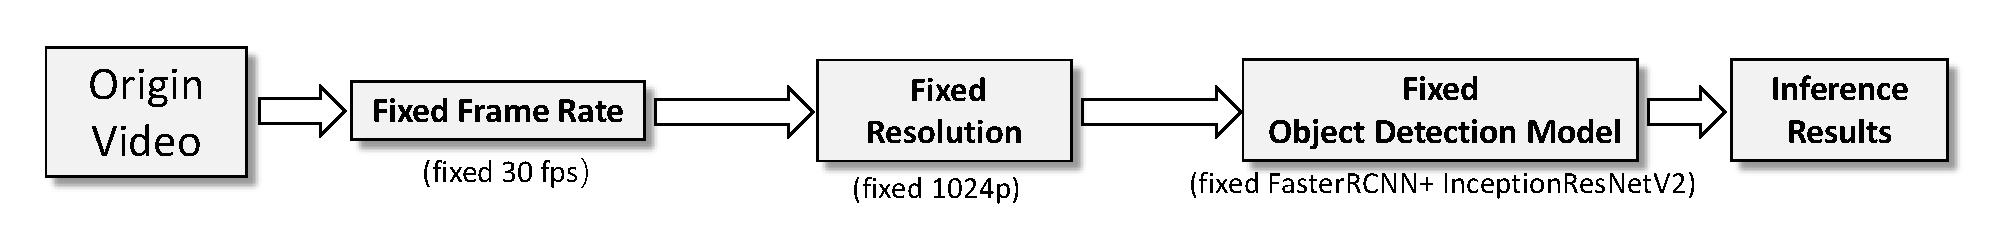
\includegraphics[width=0.9\linewidth]{figures/static_framework.pdf}}
		\begin{center}
			{(a) Static configuration solution: fixed configuration for video analytics services}
		\end{center}
		%        \vspace{0.3cm}
	\end{minipage}
	\vfill
	\vspace{0.4cm}
	\begin{minipage}{\linewidth}
		\centerline{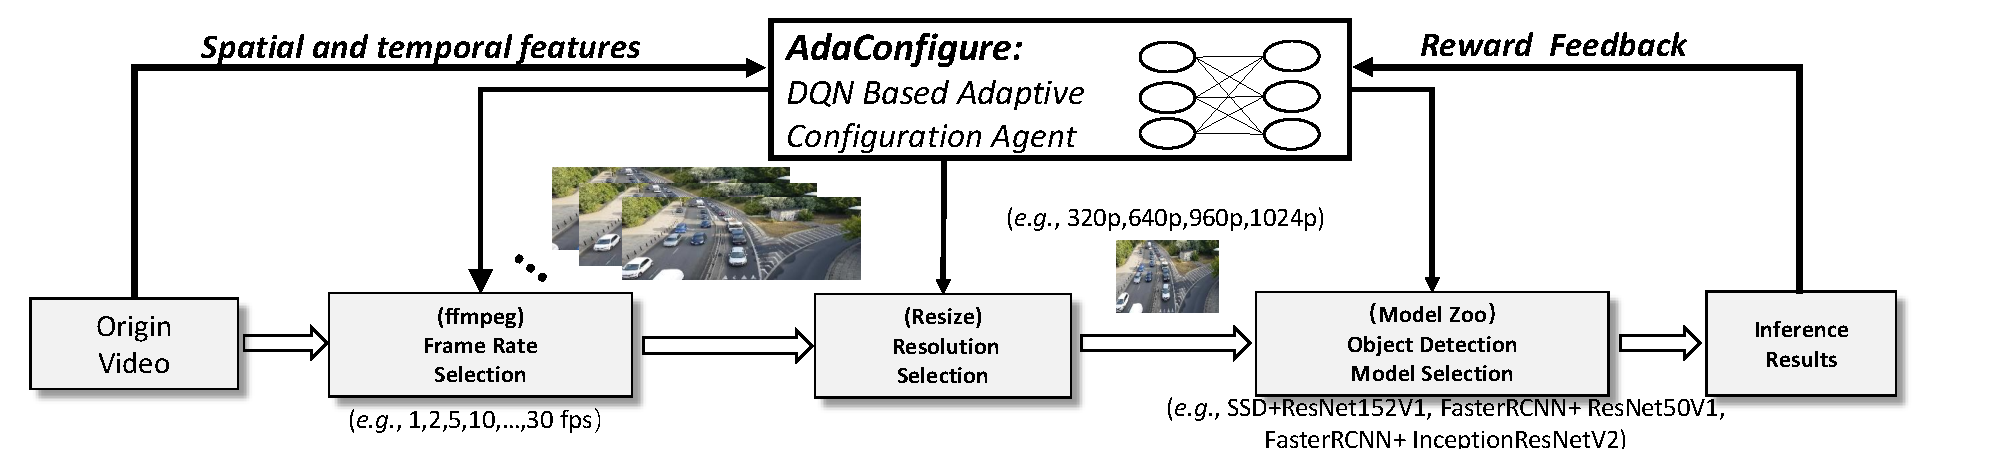
\includegraphics[width=0.9\linewidth]{figures/auto_framework.pdf}}
		\vspace{0.2cm}
		\begin{center}
			{(b) AdaConfigure solution: reinforcement learning-based adaptive configuration framework}
		\end{center}
	\end{minipage}
	%\end{tabular}
	%\vspace{0.1cm}
	\caption{Comparing to the static solution, our solution can adaptively update the configuration strategy based on the object detection model feedback}
	%	\caption{Comparing to the static solution, our solution can update the configuration strategy based on the object detection model feedback}
	\label{fig: framework}
\end{figure*}

\begin{itemize}	
	\item \emph{Choosing the best configuration is a complicated decision-making problem that is challenging to be solved by rules.} The best configuration for video analytics services changes significantly because the exact context of the videos varies over time and across space. For instance, tracking vehicles when traffic moves quickly requires a higher frame rate than when traffic moves slowly. Spatially, the characteristics of video content are different in different locations. For instance, cameras in downtown areas show more cars than the other cameras deployed in the suburbs. It is hard to make an exact rule to choose a configuration for the current context by profiling such complicated video characteristics.
%	but each condition may vary by hour, minute, even second.
	%As a dynamic video analytics configuration %solution
	%application, we target to provide a solution that dynamically picks a configuration according to intrusive dynamics of video contexts, i.e., it can \emph{generate} video analytics configuration for video analytics in a different time.
	
	\item \emph{Adaptive configuration would cause a huge extra overhead.} %The number of possible configurations grows exponentially, 
	There are thousands of configurations can be combined with just a few knobs \cite{jiang2018chameleon}. So exhaustive periodically (e.g., profile once per 4 seconds) configuration to find the best configuration is a highly unrealistic approach because it causes a huge extra overhead, which may exceed the benefits of adaptive configurations. To significantly reduce the resource cost for adaptive configuration profiling requires one solution that automaticly choose a configuration instead of manually trying using various configurations, which is challengling to previous studies including \cite{wang2020jcab,jiang2018chameleon}, since their approaches pay attention to reduce search space algorithm and still try using various configurations to find the best configuration. 
	
	%We leverage a Reinforcement Learning-based agent to adaptively pick the best configuration periodically, dramatically reducing the profiling cost. 
	%How to significantly reduce the resource cost of periodic configuration profiling.
	
	%\item \emph{Lack of well-labeled training data.} In our case, there was no well-marked data that indicated which configuration should be choosed at which time of the video, as is the case with traditional deep learning tasks.%In our problem, one is not provided the well-labeled data on which configuration should be used in which time of the video, as in conventional supervised deep learning tasks. In practice, such a video analytics configuration is usually utilized online, and the solution has to adaptively learn from the video contexts. 
\end{itemize}

%To address the above problems, 
%To address the above complicated decision-making problem and reduce the huge extra overhead of manually trying using various configurations,
%We carefully design an adaptive configuration framework based on reinforcement learning, which is an excellent approach to solve this unsupervised complex-environmental problem. 
In our solution, AutoConfigure can adaptively and automatically select the best configuration according to intrusive dynamics of video contexts, thus solving this difficult optimal configuration decision problem in a low-cost way. To the best of our knowledge, we are the first to propose an adaptive video configuration solution for such problems. 
%that adaptively and automatically chooses a configuration according to the current video context. 
The main contributions of this paper are summarized as follows. 

\begin{itemize}	
	\item We propose a Deep Q-learning Network-based \cite{DQN} agent to adaptively pick the best video analytics configuration according to the characteristics of the video stream. For the agent's state, we extract the spatial and temporal features of the video context, so that the agent can adaptively update configuration over time and achieve a superior performance in the multi-camera situation. 
	
	\item To reduce profiling cost, we leverage a video segmentation strategy and the extremely short choosing action time of agent. In particular, we divide the video into $T$-second intervals as video chunks and use the agent to choose the best configuration for the first t seconds of the video chunk, and then sticks with the chosen configuration for the rest of the video chunk ($T-t$ seconds).
%to capture the characteristics of the video stream with much-reduced computation cost: profiling a segment uses only 0.2-2\% computation resource as compared to a full video.
%	Also, we define the elements of the RL-based approach, such as actions, states, and rewards, to decide the configuration for the current video context.
	
	\item For the agent's reward, we carefully consider both inference accuracy and computation resources to assess each configuration's impact. Also, to meet different accuracy-demand services, we leverage the balance factor in the reward function to train different agents. Our solution can adaptively update configuration strategy over time, and it adaptive to different location-camera inferences and different accuracy-demand services.

% 	First, we design a reinforcement learning-based framework in which an agent adaptively chooses the configuration according to the spatial and temporal features of the current video stream.
	%	 We design an interactive training environment that can be applied to different video analytics applications.
	%	\item We build a reinforcement learning-based framework to train the agent in the above environment. The agent can learn to choose a ``most appropriate'' configuration for each timestamp of video analytics after iteratively interacting with the environment by feeding the carefully designed reward that considers both accuracy and resources.
	
%	\item We leverage dividing video strategy and the extremely short choosing action time of agent to reduce profiling cost. In the evaluation, AdaConfigure achieves 10-35\% higher accuracy with a similar amount of resources or achieves similar accuracy with only 60-90\% of the resources. Our solution proves to be more efficient than static solutions and only creates an overhead of 0.2-2\% to the overall video analytics services.
	
%	\item Our evaluation experiments on object detection task show that our approach outperforms baseline: it achieves 10-35\% higher accuracy with a similar amount of computation resources or achieves similar accuracy with only 60-90% of the computation resource. 
\end{itemize}

%The rest of this paper is organized as follows. We discuss related works in Section \ref{Section: related_works}. We present our framework and detailed design in Section \ref{Section: design}. We present our solution's performance in Section \ref{Section: evaluation} and conclude the paper in Section \ref{Section: conclusion}.

%Since video analytics applications demand intensive computation resources and high accuracy, we pay much attention to the consumption of resources in the calculation process and the inference accuracy. Therefore, the problem that follows is how to balance \emph{resource consumption} and \emph{accuracy}.

%Apparently, choosing different configurations will affect resource consumption and accuracy. When at a fixed frame rate, using a complex model with high resolution can obviously and accurately detect the target object, but it also requires more computing resources. Similarly, when using the same model with the same resolution, choosing a lower resolution can reduce the computing resources, and the subsequent cost is the decline of accuracy. When the target car (object) is large, a smaller model and a lower resolution can meet the accuracy with a considerable reduction of resource consumption, while the target car (object) is small, a more complex model and higher resolution are needed to achieve satisfactory accuracy. And in the case of highway video analytics, the rate of car travel cannot be predicted in advance, so when the car drives slowly (or static) because of the traffic jam, we can choose a lower frame rate (such as 1 FPS) instead of having to use a constant high frame rate throughout the whole video. This can significantly reduce resource consumption but does not affect the accuracy of video analytics. 


%\begin{figure*}[!t]
%	\centerline{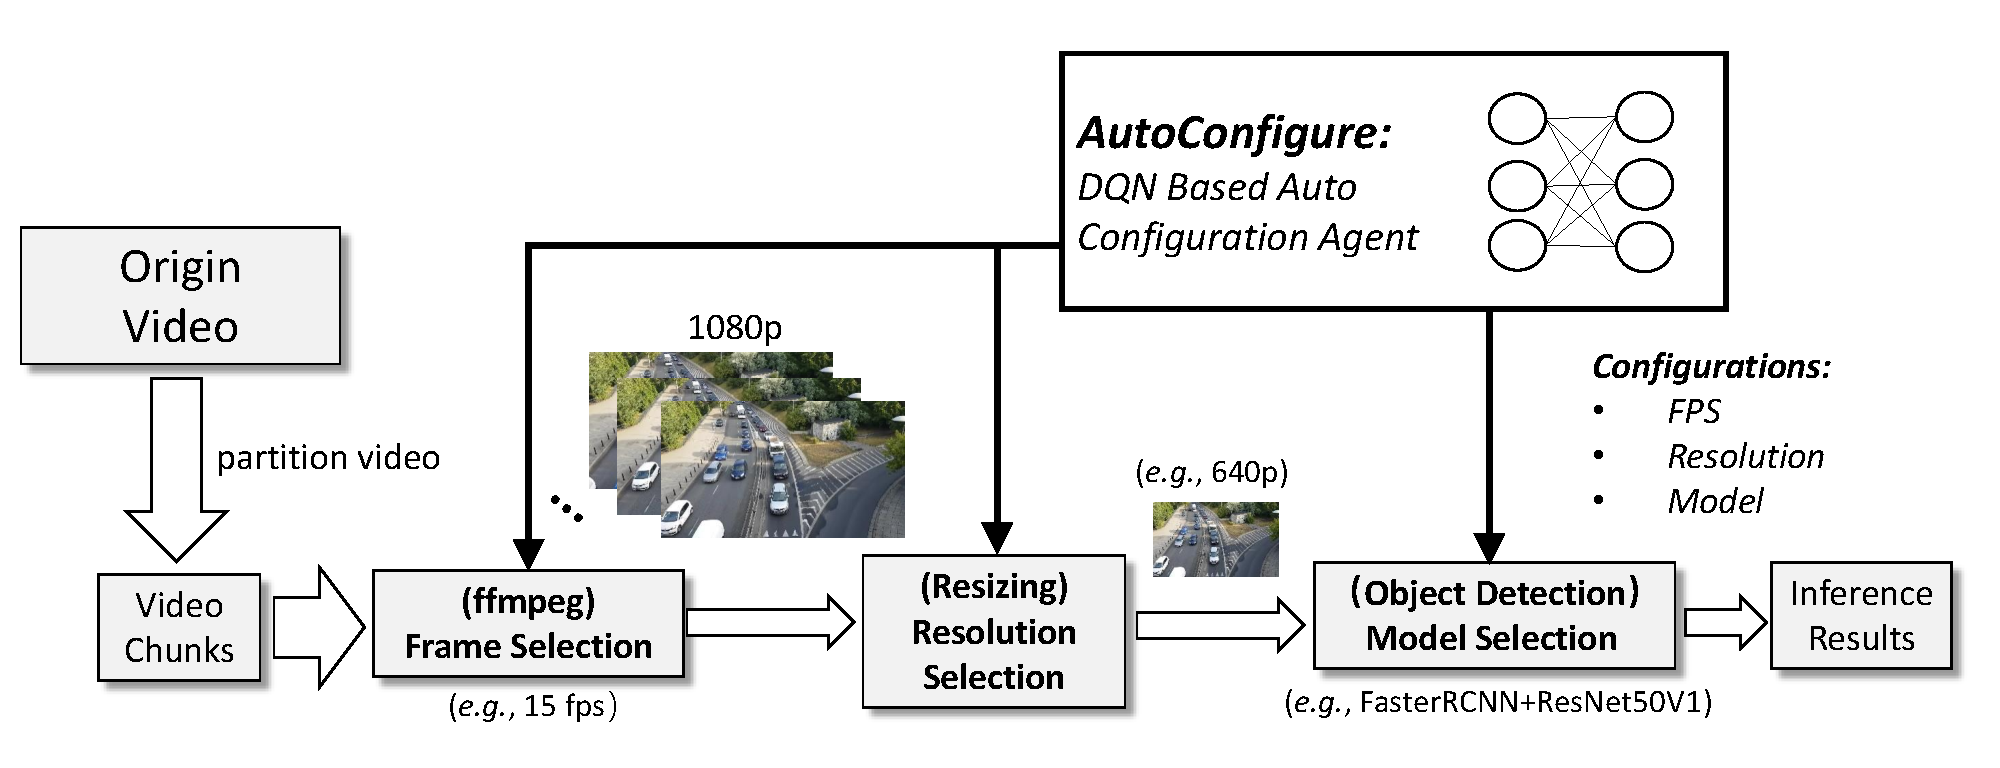
\includegraphics[width=0.9\linewidth]{figures/framework.pdf}}
%	%	\vspace{0.2cm}
%	\caption{Framework of AutoConfigure architecture}
%	\label{fig: framework}
%\end{figure*}

%We use~\autoref{fig2} to support that, the data in this figure come from a real road. It can be found that with the decrease of frame rate, the resource consumption can be significantly reduced, but the reduction of accuracy is partly acceptable.

%As shown in~\autoref{fig1}, at a fixed frame rate, using a complex model with high resolution (such as FasterRCNN+InceptionResnet 1024p) can obviously and accurately detect the target object, but it also requires more computing resources. However, when using the same model, choosing a lower resolution can reduce the computing resources, and the subsequent cost is the decline of accuracy. Another example is that choosing a simple model with low resolution (such as FasterRCNN+ResNet50 640p) can significantly reduce resource consumption, although it reduces the accuracy to some extent.

%\begin{figure}[h]
%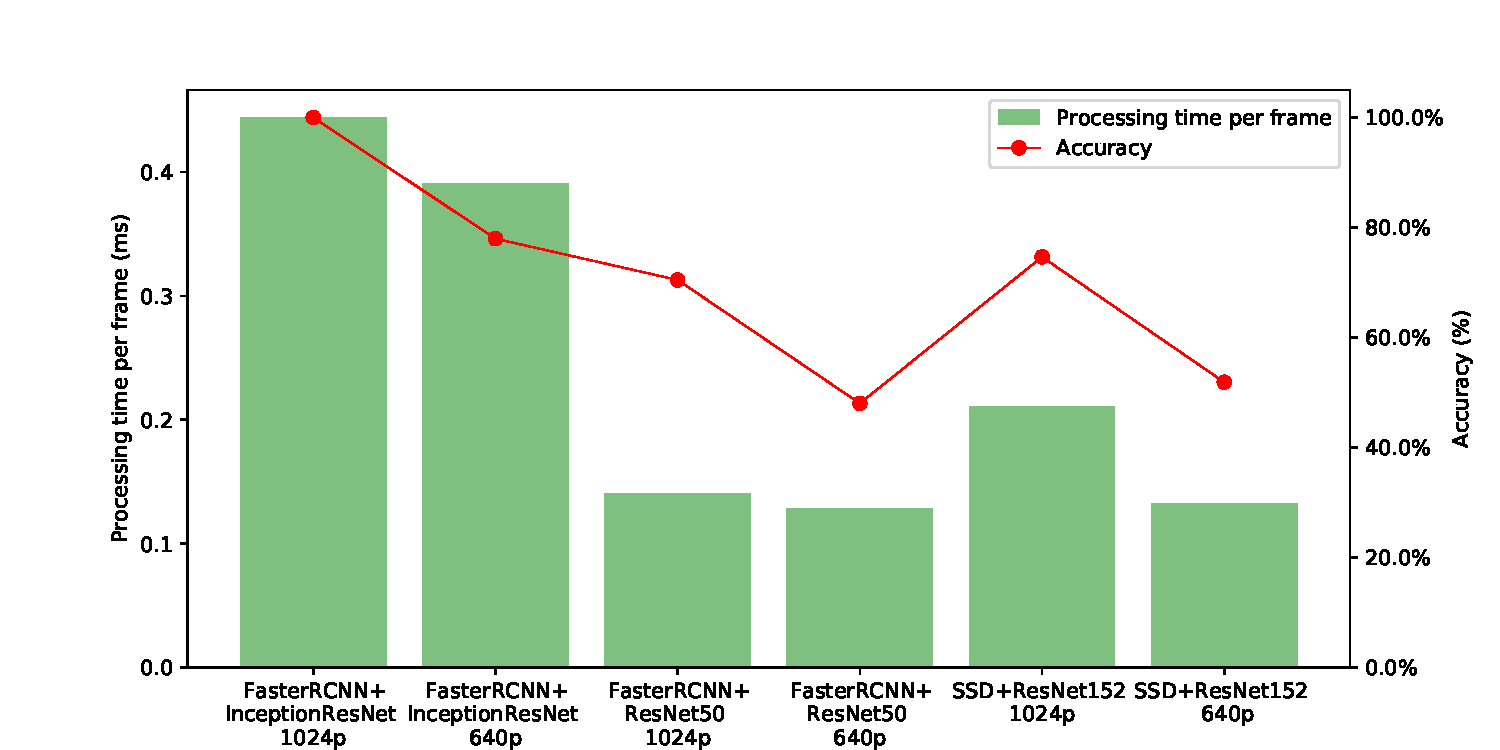
\includegraphics[width=9cm,height=5cm]{figures/figure1.pdf}
%\centering
%\caption{The effect of different models and resolutions on accuracy and processing time at a fixed frame rate.}
%\label{fig1}
%\end{figure}
%
%\begin{figure}[h]
%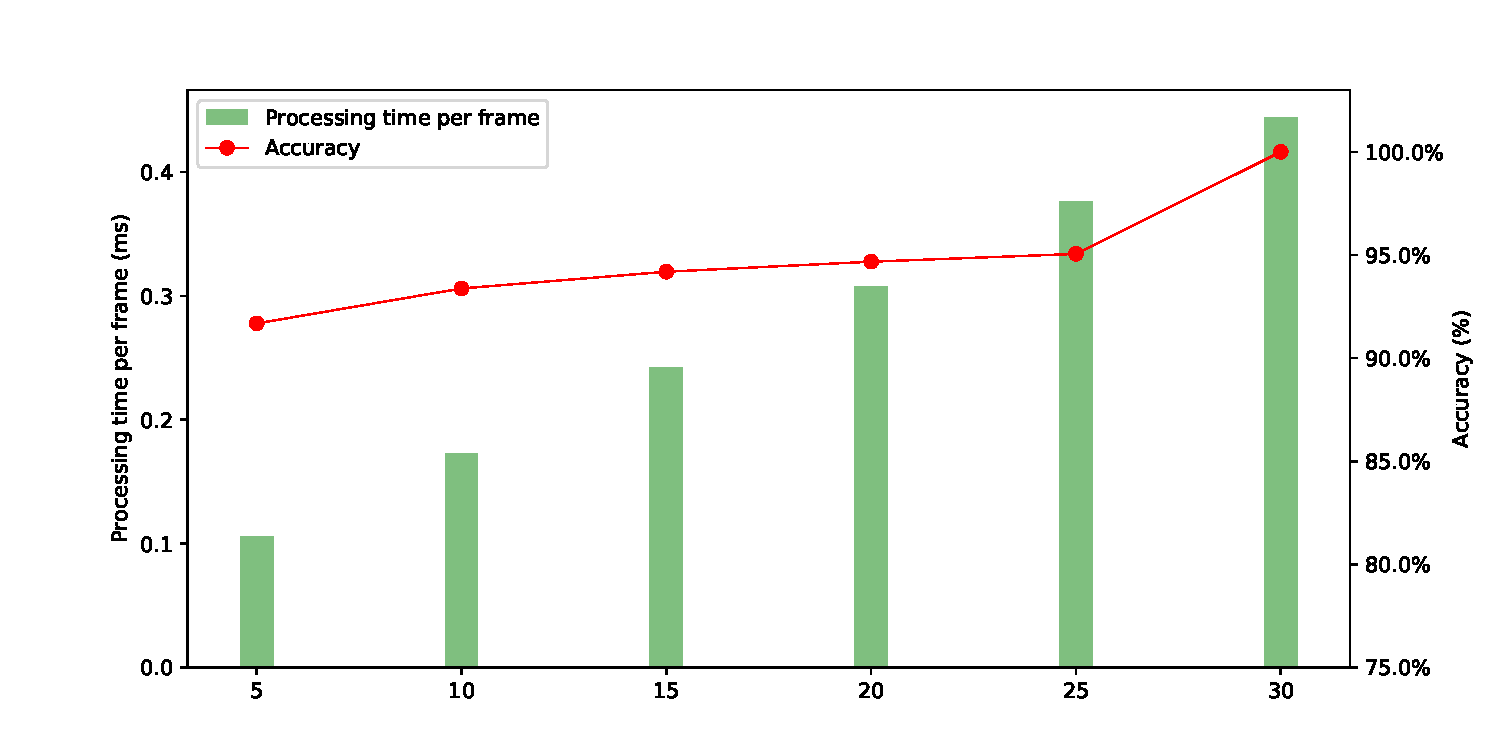
\includegraphics[width=9cm,height=5cm]{figures/figure2.pdf}
%\centering
%\caption{Under the best model, the accuracy and processing time vary with the different frame rate.}
%\label{fig2}
%\end{figure}


%Like figure~\ref{fig: framework}(a), if one just use a unified static configuration solution (i.e.only profiles the processing pipeline to choose the best configuration \emph{once}), the application would either waste resources (by picking an expensive configuration) or sacrifice accuracy (by selecting a cheap configuration).

%Hence, we aim to find a range of ``most appropriate'' configurations that %takes up the
%minimize the consumption of computing resources and is accurate to the desired threshold. On the one hand, like figure~\ref{fig: framework}(a), if one just use a unified static configuration solution (i.e.only profiles the processing pipeline to choose the best configuration \emph{once}), the application would either waste resources (by picking an expensive configuration) or sacrifice accuracy (by selecting a cheap configuration). On the other hand, if one periodically profiles the processing pipeline to find an optimal resource-accuracy \emph{tradeoff} by exhaustive all configurations, it would be prohibitively expensive since the configuration space is extremely large, and thousands of configurations can be combined with just a few knobs. To tackle these challenges, we propose an adaptive configuration approach, AutoConfigure, and the brief framework is shown in Figure~\ref{fig: framework}(b).

%The most intuitive way to solve this problem is to find the best solution by exhaustive all configurations. Still, the number of possible configurations grows exponentially, and thousands of configurations can be combined with just a few knobs, so exhaustive configuration is a highly unrealistic approach.

%For a video analytics application, choosing the ``most appropriate'' configuration is a complicated decision-making problem that is challenging to solve by rules. An adaptive approach is needed to learn from video contexts to decide the best configuration for the current video context. The reinforcement learning method is an excellent way to solve this unsupervised complex-environmental problem. In our solution, we tackle the following design challenges.


%Also, one is not provided the well-labeled data on which configuration should be used at which time of the video, meaning this is an unsupervised learning task.


\section{Related Works}
\label{Section: related_works}

\subsection{Static configuration optimization} 
Several previous papers have considered optimizing video processing pipelines by either adjusting the configuration knobs or training specialized NN models. VideoStorm \cite{zhang2017videostorm} profiles thousands of video analytics queries on live video streams over large clusters, achieving resource-quality tradeoff with multi-dimensional configurations. VideoEdge \cite{hung2018videoedge} introduces \emph{dominant demand} to identify the best tradeoff between multiple resources and accuracy, and narrows the search space by identifying a ``Pareto ban'' of promising configurations. MCDNN \cite{han2016mcdnn} provides a heuristic scheduling algorithm to adaptively select model variants of different accuracy for
deep stream processing under resource constraints. Focus \cite{hsieh2018focus} deconstructs video analytics into two phases, i.e., video ingest and video query. By tuning the share of computing resources of both phases, Focus achieves effective and flexible tradeoff of latency and accuracy of video analytics. These algorithms all profile and optimize video analytics only once at the beginning of the video. They do not handle changes in video stream content. But the optimal configurations do change over time because of the complex and changeable environment.

\subsection{Dynamic configuration optimization}
Some papers study how to dynamically optimize the configuration for video analytics when the video stream content changes.
\cite{shen2017retrain_model} adaptively retrains the NN model to detect the set of popular objects as it changes over time in the video classification task. \cite{yang2019edge_coordinated} proposes an online video quality and computing resource configuration algorithm to gradually learn the optimal configuration strategy, effectively improving the analytic accuracy while providing the low-latency response. INFaaS \cite{romero2019infaas} automatically selects a model, hardware architecture, and any compiler optimizations, and makes scaling and resource allocation decisions when application load varies and the available resources vary over time. JCAB \cite{wang2020jcab} jointly optimizes
configuration adaption and bandwidth allocation to address several critical challenges in edge-based video analytics systems,
including edge capacity limitation, unknown network variation,
intrusive dynamics of video contents. The online algorithm effectively balances analytics accuracy and energy
consumption while keeping low system latency.
 
The closest work to ours is Chameleon \cite{jiang2018chameleon}, which dynamically picks the best configurations for video analytics pipelines, reducing resource consumption
with little degradation in accuracy. They leverage temporal and spatial correlation to amortizes the cost of profiling over time and across multiple cameras, and exploit the knob independence to reduce the search space from exponential to linear. Even the search space is linear, and the profiling cost is still expensive. Such a 24-hours video, Chameleon profiles the configuration space once in every profiling window (16s), it would profile 5400 times. One profiling cost grows linear in the number of configuration knobs and the number of values per knob. The total profiling cost which is equal to one profiling cost multiply the number of profiling (5400) is also significantly high. \textcolor{note}{a little strange, can tangchen help amend?} Our solution called PerConfigure leverages a reinforcement learning-agent to choose the best configuration periodically, significantly reducing the cost of profiling since the choosing time is extremely lower. 
\section{Detailed Design}
\label{Section: design}


\begin{figure*}[!t]
	\centerline{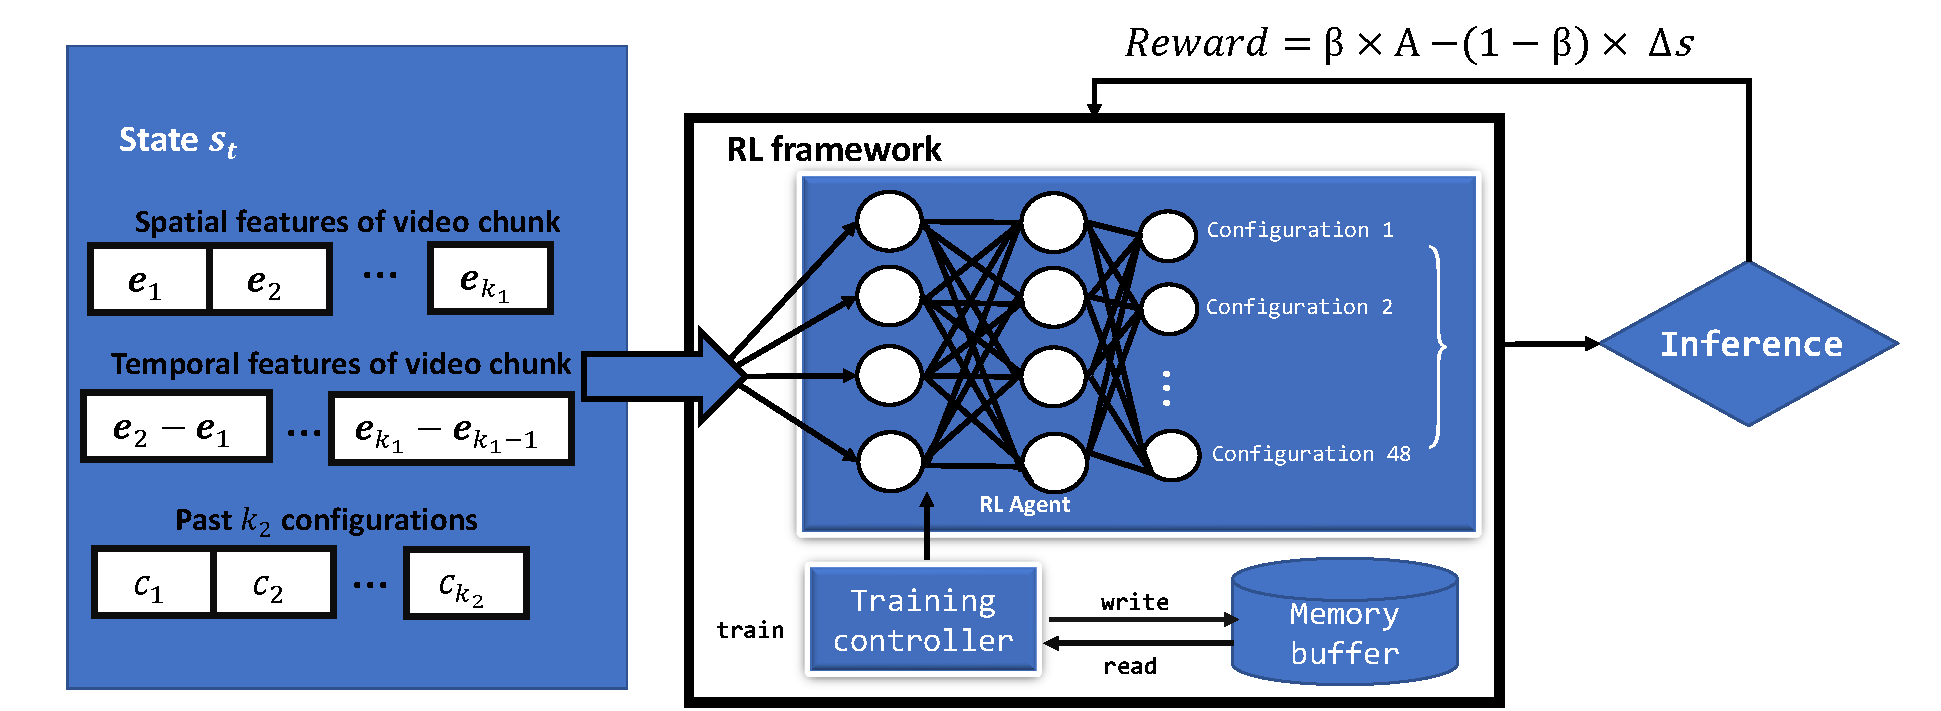
\includegraphics[width=0.9\linewidth]{figures/framework2.pdf}}
	%	\vspace{0.2cm}
	\caption{Applying reinforcement learning to adaptive configuration}
	\label{fig: DQN}
\end{figure*}

Figure~\ref{fig: DQN} summarizes how RL can be applied to the adaptive configuration. Briefly, it is a reinforcement learning-based system to train an agent to choose a proper configuration $ c $ for one video chunk to inference. We discuss the formulation, agent design, reinforcement learning-based framework, reward feedback in the following subsections. We provide experimental details of all the hyperparameters in Section~\ref{Section: experiment}. %% \\

\subsection{Problem Formulation}
\label{subsec: formulation}

To adaptively choose different configuration for video stream, we divides the video into T-second intervals as video chunks, and profiles configurations for each video chunk. Without loss of generality, we denote the object detection service as $ \vec{y}_i = M(x_i) $ that provides a predicted result list $ \vec{y}_i $ for each input video chunk $ x_i $. It has a baseline output $ \vec{y}_{\rm ref} = M(x_{\rm ref}) $ for each input video chunk $ x \in X_{\rm ref} $ using \emph{reference configuration} (the most expensive configuration). We use this $ \vec{y}_{\rm ref} $ as the ground truth label. For each video chunk $ x_c $ that uses a configuration $ c $, the output $ \vec{y}_c = M(x_c) $. Therefore, we have an accuracy metric $ \mathcal{A}_c $ by comparing $ \vec{y}_{\rm ref} $ and $ \vec{y}_c $. In general, we use the F1 score as the accuracy $ \mathcal{A} $, which is the harmonic mean of precision and recall, consistent with prior work~\cite{jiang2018chameleon,kang2017f1_noscope,zhang2017f1_live}. Besides, to compute the accuracy of a frame that was not sampled by $ c $, we use the location of objects from the previous sampled frame. 

For the cost of the object detection service, we use average GPU processing time per frame as the metric of resource consumption. We also denote the metric of resource consumption as $ \hat{s}_{ic} $ that for an input video chunk $ x_i $ and a given configuration $ c $. For a reference configuration $ c_{\rm ref} $, the reference resource consumption is $ \hat{s}_{\rm ref} $.

Initially, the agent tries different configurations $ c $ to obtain inference results image $ x_c $ from input video chunk $ x $. To obtain object detection results $ \{\vec{y}_{\rm ref}, \vec{y}_c\} $, the agent uses the choosen configuration $ c $ and the reference configuration $ x_{\rm ref} $. Comparing the two object detection results $ \{\vec{y}_{\rm ref}, \vec{y}_c\} $ and two resource consumptions $ \{\hat{s}_{\rm ref}, \hat{s}_c\} $, the agent computes the resource consumption ratio $ \Delta s = \frac{\hat{s}_c}{\hat{s}_{\rm ref}} $ and accuracy metric $ \mathcal{A}_c $.

\subsection{RL Agent Design}

The RL agent is expected to give a proper configuration $ c $ for minimizing the resource consumption $ \hat{s}_c $ while keeping the accuracy $ \mathcal{A} $. For the RL agent, the input features are continuous numerical vectors, and the expected output is discrete compression quality level $ c $. Therefore we can use the Deep Q-learning Network \cite{DQN} as the RL agent. But the naive Deep Q-learning Network can not work well in this task because the state space of reinforcement learning is too large if we directly treat video chunk as the input, making the RL agent extremely difficult to converge.  

%But the naive Deep Q-learning Network can not work well in this task because the state space of reinforcement learning is too large if we directly treat video chunk as the input. To preserve enough details, we have to add many layers and nodes to the neural network, making the RL agent extremely difficult to converge. 

%because of the following challenges: %% \\
%
%\begin{itemize}
%	\item The state space of reinforcement learning is too large. To preserve enough details, we have to add many layers and nodes to the neural network, making the RL agent extremely difficult to converge. 
%	\item It takes a long time to train one step in a large inference neural network, making the training process too time-consuming.
%	\item The RL agent starts training from random trials and learns afterward from the reward feedback. When training from a randomly initialized neural network, the reward feedback is very sparse, making it difficult for the agent to learn.
%\end{itemize}

To address this challenges, we leverage FFmpeg \cite{FFmpeg} to extract the top $k_1$ representative images from each chunk as spatial features of video chunk. We use a pre-trained small neural network to extract the structural information embeddings $ \{e_1,e_2,...,e_{k_1}\} $ of the images to reduce the input dimension and accelerate the training procedure. This is a commonly used strategy in training a deep neural network~\cite{finetunning,finetunning2}. In this work, we use the early convolution layers of MobileNetV2~\cite{MobileNetV2} as the image feature extractor $ \mathcal{E}(\cdot) $ for its efficiency in image classification. To extract the temporal features of video chunk, we obtain $ \{\hat{e}_1,\hat{e}_2,...,\hat{e}_{{k_1}-1}\} $ by each embedding subtracting previous embedding. Besides, we record the last $k_2$ configurations $ \{c_1,c_2,...,c_{k_2}\} $. To Solve that vectors of different lengths are not conducive to input to the neural network, we use fully connected layer to transform the spatial embedding $ \{e_1,e_2,...,e_{k_1}\} $, temporal embedding $ \{\hat{e}_1,\hat{e}_2,...,\hat{e}_{{k_1}-1}\} $, and recent configuration $ \{c_1,c_2,...,c_{k_2}\} $ to the fixed length vector, similar to the work~\cite{pensieve}. We formulate the fixed length vector $ s $ as \emph{states} and the configuration $ c $ as discrete \emph{actions}.

\subsection{Reinforcement Learning-based Framework}

In our system, we define 48 discrete actions to indicate 48 configuration, and the specific configurations are provided in Section~\ref{subsec: configuration}. We denote the \emph{action-value function} as $ Q(s, c; \theta) $ and the optimal compression quality level at time $ t $ as $  c_t = {\rm argmax}_cQ(s, c; \theta) $ where $ \theta $ indicates the parameters of the Deep Q-learning Network $ \phi $. In such reinforcement learning formulation, the training phase is to minimize the loss function $ L_i(\theta_i) = \mathbb{E}_{s, c \sim \rho (\cdot)}\Big[\big(y_i - Q(s, c; \theta_i)\big)^2 \Big] $ that changes at each iteration $ i $ where target $ y_i = \mathbb{E}_{s' \sim \{\mathcal{X}, M\}} \big[ r + \gamma \max_{c'} Q(s', c'; \theta_{i-1}) \mid s, c \big] $. Especially, $ r $ is the reward feedback, and $ \rho(s, c) $ is a probability distribution over state  $ s $ and the configuration $ c $~\cite{DQN}. When minimizing the distance of \emph{action-value function}'s output $ Q(\cdot) $ and target $ y_i $, the \emph{action-value function} $ Q(\cdot) $ outputs a more accurate estimation of an action. 

In the training phase, the RL agent firstly using an $\epsilon-$greedy method to take some random trials to observe the environment's reaction and decreases the randomness when training afterward. In iteration $t$, we input state $s_t $ to neural network $ \phi $. The RL agent $\phi$ generates a specific configuration $c_t$. The framework processes the video chunk $x_t$ using configuration $c_t$ to inference object detection services and obtains reward $r_t$. Then the framework obtains the next video chunk $x_{t+1}$ and generates the next state $ s_{t+1} $. The framework stores transition $(s_t, c_t, r_t, s_{t+1})$ in a memory buffer $\mathcal{D}$. Especially, the transition $(s_t, c_t, r_t, s_{t+1} )$ is uesd to compute the loss function. All transitions are saved into a memory buffer $ \mathcal{D} $, and the agent learns to optimize its \emph{action} by minimizing the loss function $ L $ on a mini-batch from $ \mathcal{D} $. The training procedure would converge when the agent's randomness keeps decaying. Finally, the agent's action is based on its historical ``optimal'' experiences. The training procedure is presented in Algorithm~\ref{alg: rl-train}.

\begin{algorithm}[!t]
		\caption{Training RL agent $ \phi $} %in environment $ \{\mathcal{X}, M\} $}
		\label{alg: rl-train}
		\begin{algorithmic}[1]	
			\STATE Initialize action-value function $ Q $ with random weights $ \theta $, replay memory buffer $ \mathcal{D} $ and state $ s_1 $				
			\FOR {$t \in 1,2,\cdots, K$}
			\STATE \textbf{1) Exploration}
			\STATE With probability $\epsilon$:
			\STATE \hspace{1em} $c_t \leftarrow$ a random valid value 
			\STATE Otherwise:
			\STATE \hspace{1em} $ c_t \leftarrow {\rm argmax}_cQ(s_t, c; \theta) $ 

			\STATE \textbf{2) Reward calcuation} 
			\STATE Process video chunk $ x_t $ using configuration $ c_t $ to inference
			\STATE Obtain $ (\vec{y}_{\rm ref}, \vec{y}_c) $ from the object detection service
			\STATE Compute reward $ r \leftarrow R(\Delta s, \mathcal{A}_c) $ according to \ref{subsec: reward} Reward Feedback Design 
			\STATE \textbf{3) Gradient descent}
			\STATE Obtain next video chunk $ x_{t+1} $
			\STATE Generate next state $ s_{t+1} $
			\STATE $ \mathcal{D} \leftarrow \mathcal{D} \bigcup \{(s_t, c_t, r_t, s_{t+1} \} $
			\STATE Sample a randomly mini-batch of transitions $ (s_j, c_j, r_j, s_{j+1}) $ from memory buffer $ \mathcal{D} $
			\STATE $ y_j \leftarrow r_j + \gamma \max_{c'}Q(s_{j+1}, c'; \theta) $
			\STATE Perform a gradient descent step on $ \big(y_j - Q(s_j, c_j; \theta)\big)^2 $ according to~\cite{DQN}
			\ENDFOR
		\end{algorithmic}
\end{algorithm}

\subsection{Reward Feedback Design}
\label{subsec: reward}

In our solution, the agent is trained by the reward feedback. In the above formulation, we define resource consumption rate $ \Delta s = \frac{\hat{s}_c}{\hat{s}_{\rm ref}} $ and accuracy metric $ \mathcal{A}_c $ at configuration $ c $. Basically, we want the agent to choose a proper configuration for minimizing the resource consumption while remaining acceptable accuracy. Therefore the overall reward $ r $ should be positively correlated with the accuracy $ \mathcal{A} $ while negatively with the resource consumption ratio $ \Delta s $. We introduce a balance factor $ \beta $ to form a linear combination $ r = \beta \mathcal{A} - (1-\beta) \Delta s  $ as the \emph{reward function} $ R(\Delta s, \mathcal{A}) $. %% \\

%\section{Evaluation}
\label{Section: evaluation}

\subsection{Experiment Setup}

\subsection{some results}

%\begin{table}[!t]
%\begin{table}[H]
%	\centering
%	%     \begin{tabular}{lll}
%	\resizebox{0.5\textwidth}{!}{
%	\begin{tabular}{lcc}
%		\toprule
%		Model and Image size & Inference time & Accuracy  \\ \midrule
%		SSD MobileNetV2 320p          & 49.5 ms  &  xxx            \\
%		SSD MobileNetV2 640p          & 58.5 ms  &  0.494            \\
%		SSD ResNet152V1 640p          & 100 ms  &  0.579            \\
%		SSD ResNet152V1 1024p          & 182.3 ms  &  0.614            \\
%		FasterRCNN ResNet50V1 640p          & 106.4 ms  &  0.637            \\
%		FasterRCNN ResNet50V1 1024p          & 120.5 ms  &  0.786           \\
%		FasterRCNN InceptionResNetV2 640p          & 361.8 ms  &  0.734            \\
%		FasterRCNN InceptionResNetV2 1024p          & 418.4 ms  &  1            \\
%		\bottomrule
%	\end{tabular}}
%	\caption{Inference time and F1 for different models and resolutions}
%	\label{tab: latency-overhead}
%	% \vspace{-0.5cm}
%\end{table}

%\begin{table}[!t]
\begin{table}[H]
	\centering
	%     \begin{tabular}{lll}
	\resizebox{0.5\textwidth}{!}{
		\begin{tabular}{lcc}
			\toprule
			Model and Image size & Inference time & Accuracy  \\ \midrule
			SSD MobileNetV2 320p          & 49.5 ms  &  xxx            \\
			SSD MobileNetV2 640p          & 58.5 ms  &  0.753            \\
			SSD ResNet152V1 640p          & 100 ms  &  0.886            \\
			SSD ResNet152V1 1024p          & 182.3 ms  &  0.942            \\
			FasterRCNN ResNet50V1 640p          & 106.4 ms  &  0.889            \\
			FasterRCNN ResNet50V1 1024p          & 120.5 ms  &  0.98           \\
			FasterRCNN InceptionResNetV2 640p          & 361.8 ms  &  0.965            \\
			FasterRCNN InceptionResNetV2 1024p          & 418.4 ms  &  1            \\
			\bottomrule
	\end{tabular}}
	\caption{Inference time and F1 for different models and resolutions}
	\label{tab: latency-overhead}
	% \vspace{-0.5cm}
\end{table}
\section{Evaluation}
\label{Section: experiment}

\subsection{Experiment Setup and Configuration Selection}
\label{subsec: configuration}
We carry out real-world experiments on the object detection task (basic computer vision services) to verify our solution’s performance. We use a desktop PC (Intel Xeon E5-2650 v4 CPU) with four NVIDIA 1080ti graphic card as the server infrastructure, and simulate the environment \cite{trade-offs} with three pretrained object detection models in Tensorflow, which are SSD+ResNet152V1, FasterRCNN+ResNet50V1, FasterRCNN+InceptionResNetV2. For each model, two kinds of image resolution, which is $1024\times1024$ and $640\times640$, can be picked up. In our experiment, we set the choices space of fps as \{1, 2, 5, 10, 15, 20, 25, 30\}. We use FFmpeg to switch the frame rate and image resolution, which decide which frames and in what size they should be fed to the object detection model. The configuration space comprises all possible combinations of values of these knobs, so the environment has 48 configurations in total.
%In the service inference, the processing video module uses CPU resources, and the object detection module uses GPU resources. In our study, we use GPU processing time as the metric of resource consumption because GPU is the dominant resource for most video processing workloads \cite{jiang2018chameleon}.In the evaluation, the processing video module needs 62s to decode 5 mins video into 9000 frames image (i.e., average CPU processing time per frame is about 0.006s), which is lower than the GPU processing time. To reduce the latency of processing video, we use different processes to carry out the processing video module and the object detection module in our experiments.   

\subsection{Dataset and Metric}
\label{subsec: datasets}
Most public sources datasets cannot fully satisfy all configuration choices, they provide only a fraction of the requirements for configuration. %for example, some can only guarantee 30 frames but cannot guarantee 1024p resolution. In contrast, others can ensure resolution but cannot provide a sufficient frame rate. 
%In recent years, most of the driving recorder can provide enough resolution and frame rate, so 
We try to search keywords (e.g., ``highway traffic'') on Youtube and download videos that meet the resolution and frame rate requirements. We selecte three datasets: M6, Duke, and Multi-Camera Dataset. M6 is taken from a traffic camera on the longest motorway in Britain. Duke is a video from a fixed camera placed at an intersection, and the traffic flow in the video increases or decreases periodically with the traffic light change. 
%Since the first two datasets were sourced from a fixed camera, 
To ensure that AdaConfigure performs better in multi-camera inference, we combine three videos collected from different locations into one video dataset, Multi-Camera Dataset. The exact content of this dataset varies significantly over time and across space.

For metric, we use the F1 score as the accuracy and average GPU processing time per frame as the resource consumption because GPU is the dominant resource for most video processing workloads \cite{jiang2018chameleon}. F1 score is the harmonic mean of precision and recall, where the precision is true positives divided by the detected objects, and the recall is true positives divided by the ground truth objects. We identify true positives using two conditions, an abounding box-based condition (only check the classified label) and a label-based condition (check the classified label and spatial overlap \cite{overlap}), consistent with prior work \cite{jiang2018chameleon,noscope}. Both accuracy metrics are useful in real video analytics services and used in our experiments. Besides, to compute the accuracy of a frame that is not sampled by exact configuration, we use the location of objects from the previous sampled frame. 
%described in Section \ref{subsec: formulation}.
%, consistent with prior work [24, 32].
%First, to eliminate the bias caused by Cookies and personal preferences, we use private browsing mode to search keywords (e.g., "drivecam highway hd"). Second, manually delete irrelevant videos (e.g., ads for some driving recorders) and download videos that are longer than ten minutes. These videos need to be as dynamic as the real world, such as not standing still for too long. Because none of these videos contained ground truth, we used the original video output data from DNN as the tags to calculate the accuracy. For instance, in object detection, the accuracy is defined by the F1 score with respect to the server-side DNN output in highest resolution (original) with over 50$\%$ confidence score.Based on the above filtering strategy, we finally selected three datasets: 

%we selected three datasets:
%M6: The M6 is the longest motorway in Britain and the most important road from the Midlands to the West Coast. Thousands of cars travel on it every day. This video was taken from a traffic camera, and its natural dynamics allows us to experiment with this video.
%
%Duke: Duke is a video from a fixed camera placed at an intersection. Because it is fixed in the middle of the intersection, the traffic flow in the video increases or decreases periodically as the traffic light change.
%
%Mutli Camera Dataset: Since the first two datasets were sourced from a fixed camera, in order to ensure that AdaConfigure still has better performance when road conditions change dramatically, we used three videos collected from the dashcam, and since they are relatively similar, we combined them into one video.

%\begin{figure*}[!t]
%	\begin{minipage}[t]{0.32\linewidth}
%		\centerline{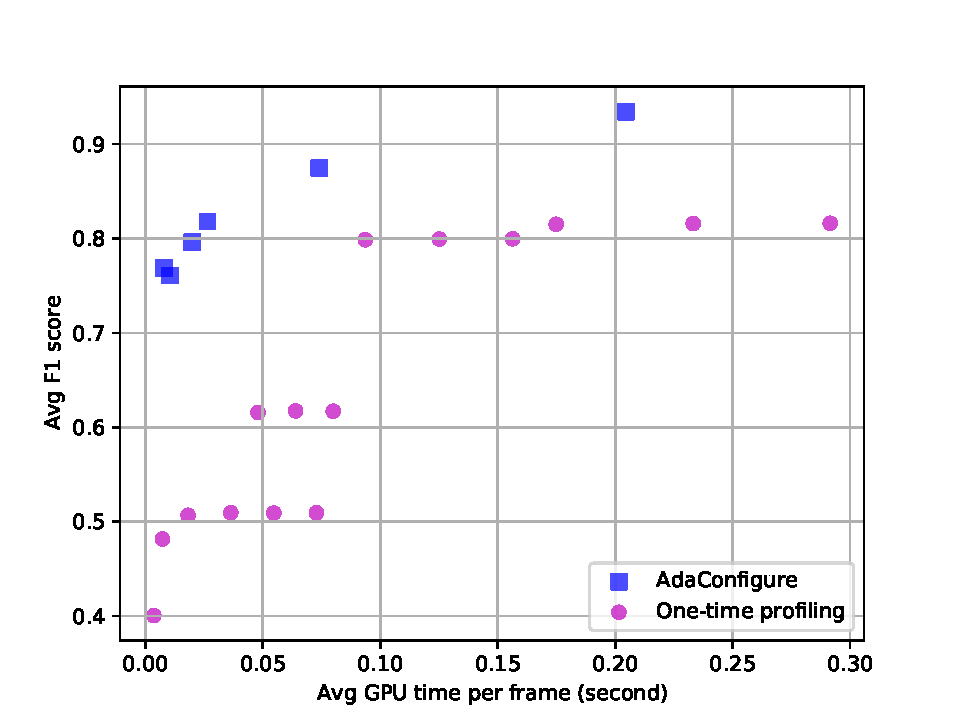
\includegraphics[width=6.5cm]{figures/m6.pdf}}
%		\centerline{(a) M6 (Bounding box-based)}
%	\end{minipage}
%	\hfill
%	\begin{minipage}[t]{0.32\linewidth}
%		\centerline{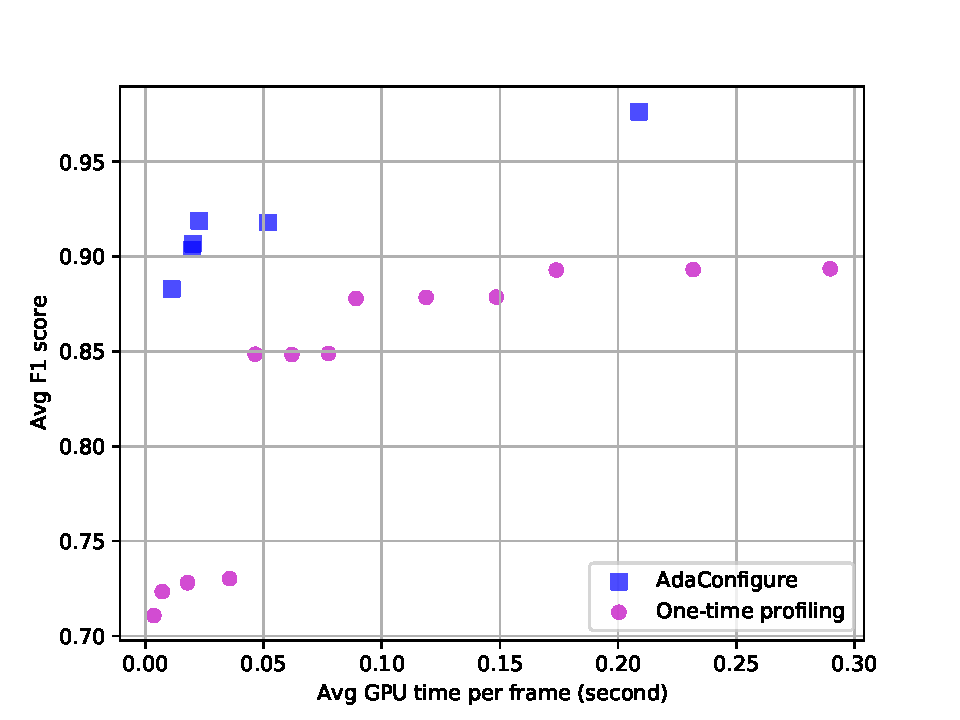
\includegraphics[width=6.5cm]{figures/duke.pdf}}
%		\centerline{(b) Duke (Bounding box-based)}
%	\end{minipage}
%	\hfill
%	\begin{minipage}[t]{0.32\linewidth}
%		\centerline{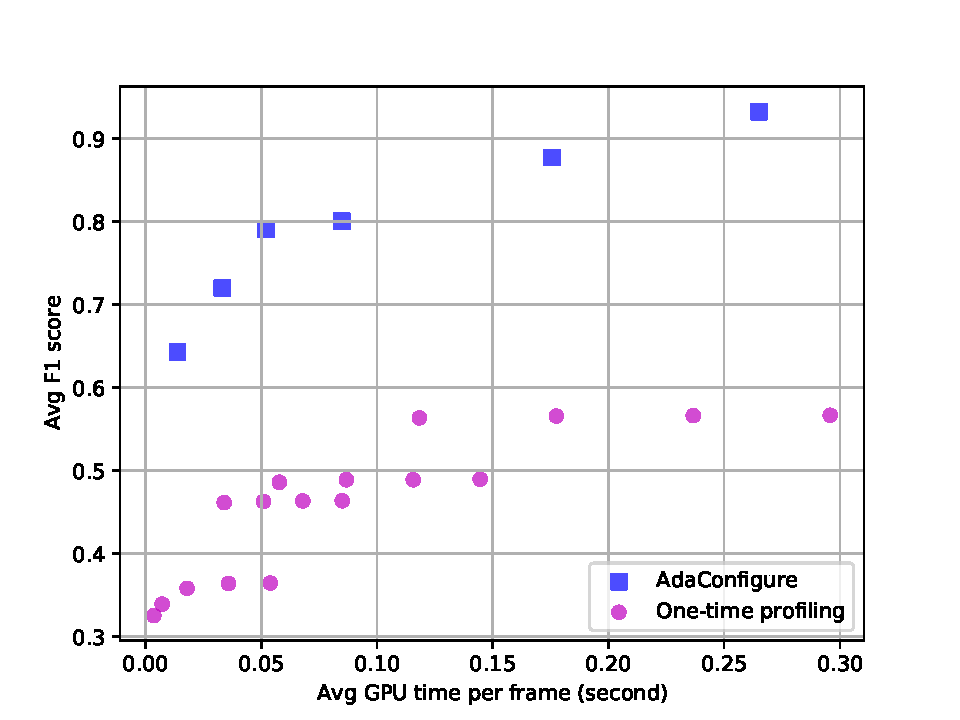
\includegraphics[width=6.5cm]{figures/_Westbound_Eastbound_Rear.pdf}}
%		\centerline{(c) Multi-Camera Dataset (Bounding box-based)}
%	\end{minipage}
%	\vfill
%%	\vspace{0.4cm}
%	\begin{minipage}[t]{0.32\linewidth}
%		\centerline{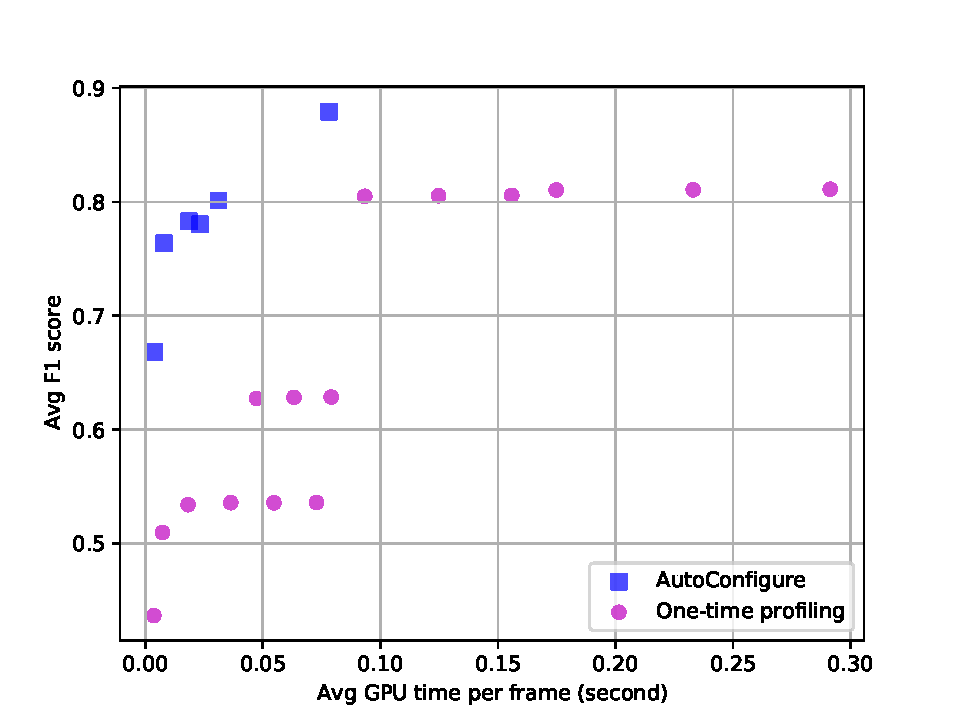
\includegraphics[width=6.5cm]{figures/m6_label.pdf}}
%		\centerline{(d) M6 (label-based)}
%	\end{minipage}
%	\hfill
%	\begin{minipage}[t]{0.32\linewidth}
%		\centerline{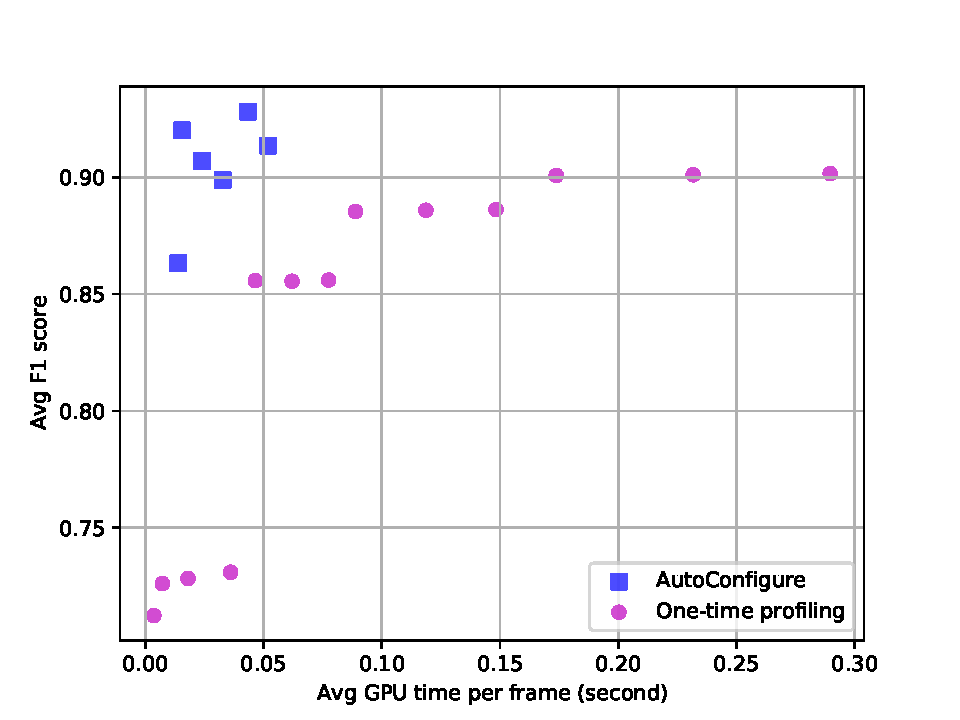
\includegraphics[width=6.5cm]{figures/duke_label.pdf}}
%		\centerline{(e) Duke (label-based)}
%	\end{minipage}
%	\hfill
%	\begin{minipage}[t]{0.32\linewidth}
%		\centerline{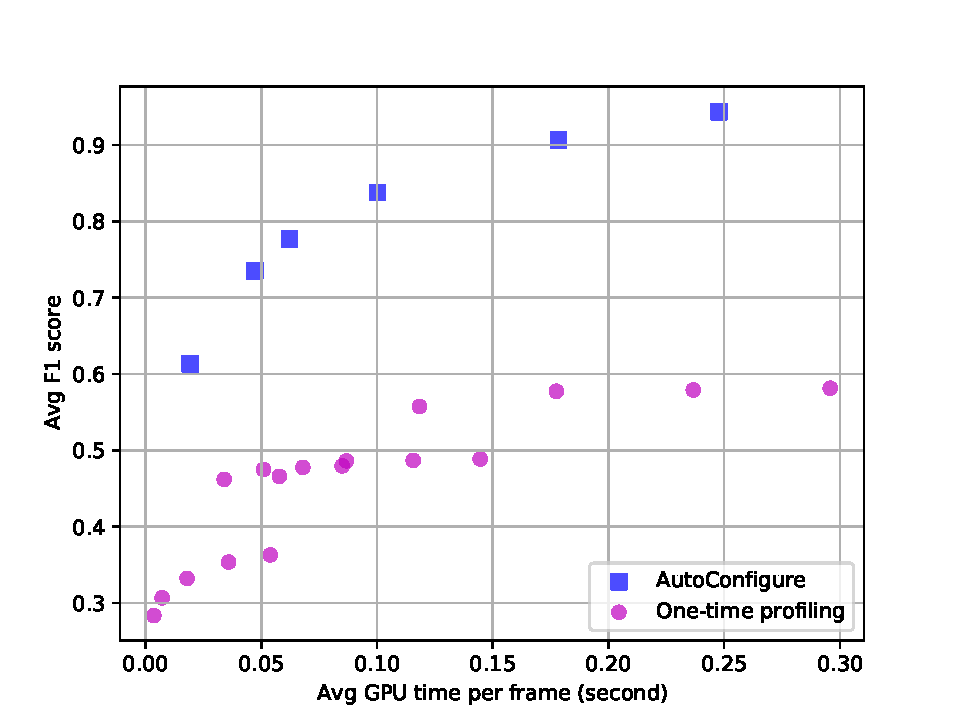
\includegraphics[width=6.5cm]{figures/_Westbound_Eastbound_Rear_label.pdf}}
%		\centerline{(f) Multi-Camera Dataset (label-based)}
%	\end{minipage}		
%	\caption{AdaConfigure (blue) consistently outperforms the baseline of one-time profiling (magenta) across different metrics on different datasets. Each dot represents the results of running each solution.}
%	\label{fig: results}
%\end{figure*}

\begin{figure}[!t]
	\begin{minipage}[t]{0.47\linewidth}
	\centerline{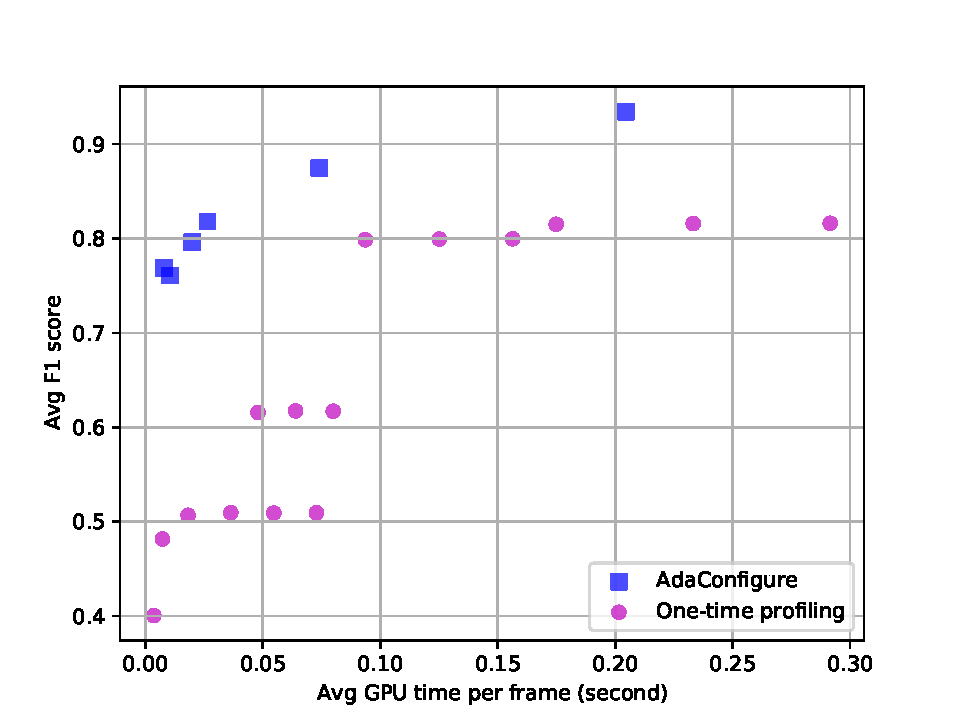
\includegraphics[width=5cm]{figures/m6.pdf}}
	\centerline{(a) M6 (Bounding box-based)}
	\end{minipage}
	\hfill
	\begin{minipage}[t]{0.47\linewidth}
	\centerline{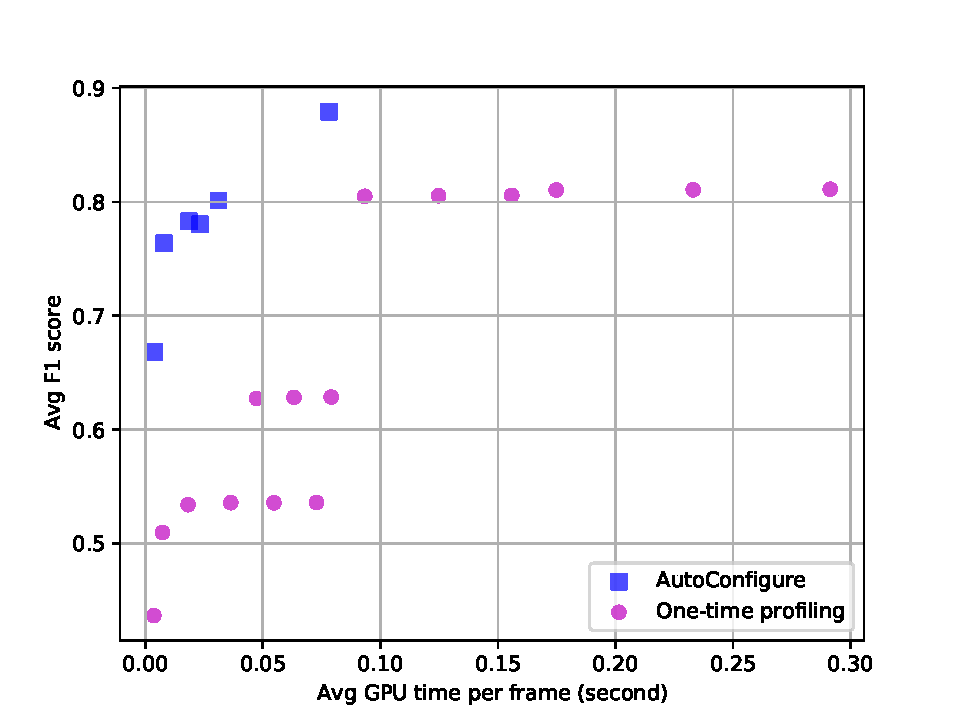
\includegraphics[width=5cm]{figures/m6_label.pdf}}
	\centerline{(b) M6 (label-based)}
	\end{minipage}
	\vfill
	\begin{minipage}[t]{0.47\linewidth}
	\centerline{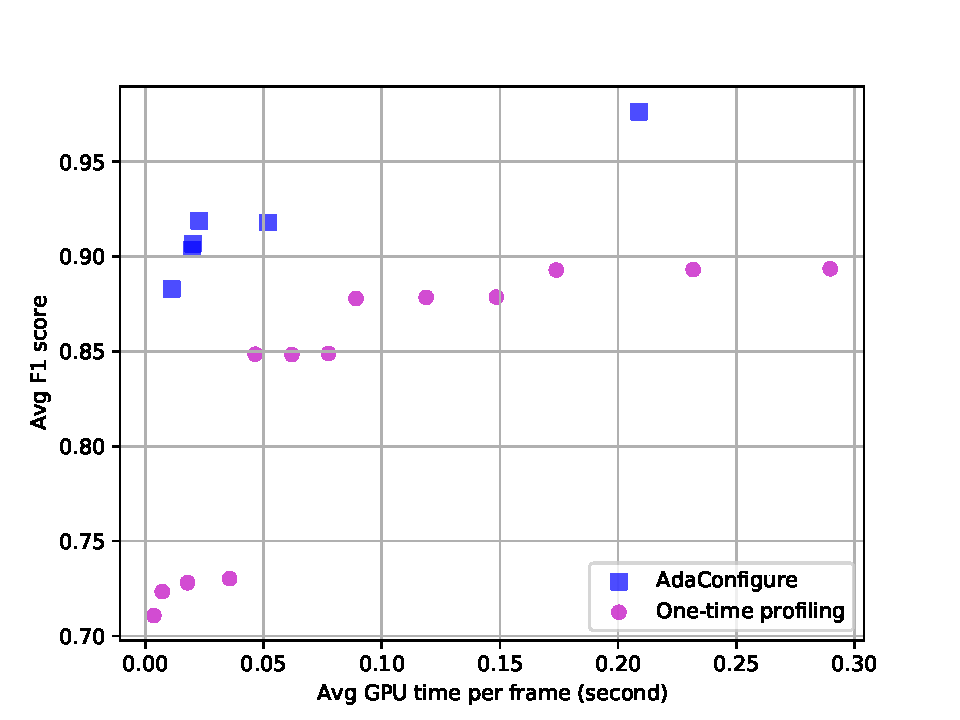
\includegraphics[width=5cm]{figures/duke.pdf}}
	\centerline{(c) Duke (Bounding box-based)}
	\end{minipage}
	\hfill
	%	\vspace{0.4cm}
	\begin{minipage}[t]{0.47\linewidth}
	\centerline{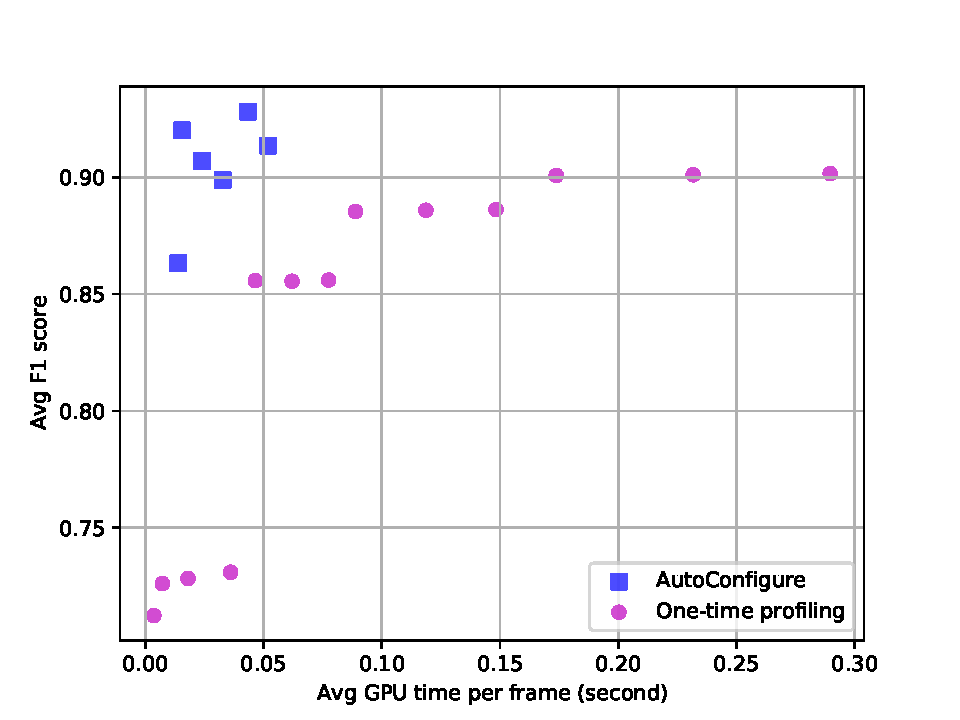
\includegraphics[width=5cm]{figures/duke_label.pdf}}
	\centerline{(d) Duke (label-based)}
	\end{minipage}
	\vfill
	\begin{minipage}[t]{0.47\linewidth}
	\centerline{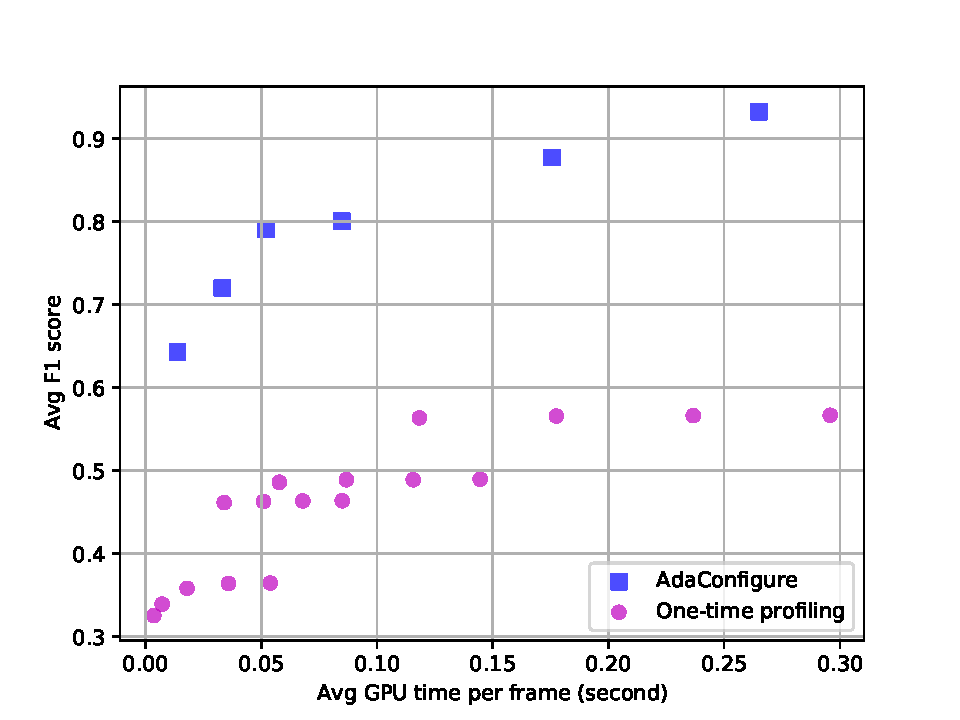
\includegraphics[width=5cm]{figures/_Westbound_Eastbound_Rear.pdf}}
	\centerline{(e) Multi-Camera Dataset }%\\ (Bounding box-based)}
	\centerline{(Bounding box-based)}
	\end{minipage}
	\hfill
	\begin{minipage}[t]{0.47\linewidth}
	\centerline{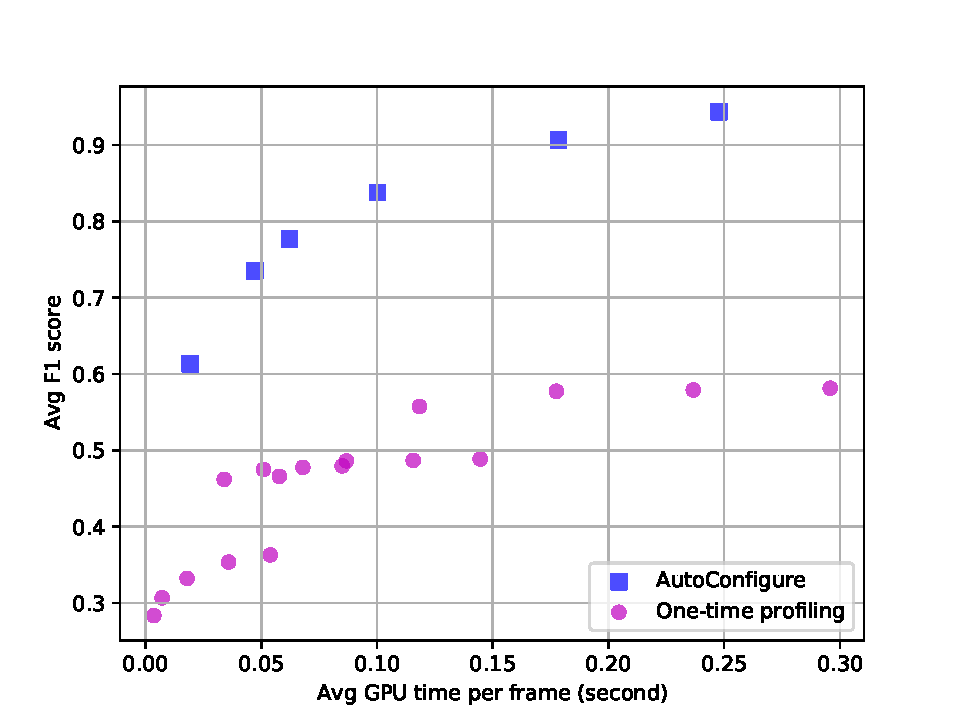
\includegraphics[width=5cm]{figures/_Westbound_Eastbound_Rear_label.pdf}}
	\centerline{(f) Multi-Camera Dataset }% (label-based)}
	\centerline{(label-based)}
	\end{minipage}		
	\caption{AdaConfigure (blue) consistently outperforms the baseline of one-time profiling (magenta) across different metrics on different datasets. Each dot represents the results of running each solution.}
	\label{fig: results}
%	\vspace{-0.5cm} 
\end{figure}

\subsection{Experiment Parameters}
%We apply a deep Q-learning network policy to train the agent. 
In the training procedure, we build up to eight independently identical environments for each data set to speed up the training and decrease the data's dependency. For each dataset, we train the agent 5 epochs and 600 steps (5 mins) per epoch. Some important hyperparameters in our experiments are given in Table ~\ref{tab: parameters}.
%The leaning rate is set to 0.001.

\begin{table}[!t]
	\centering
	%     \begin{tabular}{llllll}
	\resizebox{0.4\textwidth}{!}{
		\begin{tabular}{cccccc}
			\toprule
			Notation          & Value & & & Notation     & Value  \\ \midrule
			$\epsilon$    & 0.8    & & & $k_1$      & 3   \\
			$\gamma$      & 0.9  & & & $k_2$    & 3    \\
			$ \beta $ & 0.2,0.3,...,0.7 & & & $ T (train) $ & 1  \\
			$ t(inference)  $  &  1   & & &   $ T (inference)  $  &  4      \\ 
			\bottomrule
	\end{tabular}}
	\caption{Experiment parameters}
	\label{tab: parameters}
%	\vspace{-0.5cm}
\end{table}

\subsection{Experiment Results}
%We use bounding box-based and label-based metric to evaluate AdaConfigure on M6, Duke, and Multi-Camera Dataset video streams. at the beginning of a video stream \{SSD+ResNet152V1, 640p, 2fps\},
Figure \ref{fig: results} shows that AdaConfigure consistently outperforms the static configuration baseline (only profiling configurations once) along with resource consumption and two accuracy metrics on different datasets. Each magenta dot represents one static configuration solution (one-time profiling).
These static configuration solutions include some fixed expensive configurations and fixed cheap configurations. 
%These static configuration solutions include some expensive configurations, such as \{FasterRCNN+InceptionResNetV2, 640p, 30fps\}, \{FasterRCNN+ResNet50V1, 1024p, 25fps\}, and some cheap configurations, such as \{SSD+ResNet152V1, 640p, 1fps\}, \{SSD+ResNet152V1, 640p, 5fps\}.
Each blue dot represents one AdaConfigure configuration solution, which is dependent on the balance factor $\beta$ in reward function, presented in Section \ref{subsec: reward}. The detailed discussion about different AdaConfigure solutions is in Section \ref{subsec: different sulutions}. Note that AdaConfigure's resource consumption includes both running the best configuration to get inference results and profiling cost of adaptive configuration, which detailed discussed in \ref{subsec: profiling cost}. 

As shown in Figure \ref{fig: results}, Adaconfigure achieves a high accuracy of 10-35\% with the same amount of computing resources, which benefits from the adaptive selection of relatively expensive configuration when the video content is complex (e.g., traffic congestion, high-speed vehicles). Also, Adaconfigure achieves a 50-90\% reduction in resource consumption while achieving almost the same precision as the baseline, which benefits from the adaptive selection of relatively cheap configurations when the video content is simple (e.g., low-traffic flow).

%As shown in Figure \ref{fig: results}, Adaconfigure achieves a high accuracy of 10-35\% with a similar amount of computing resources or achieves a 50-90\% reduction in resource consumption while achieving almost the same precision as the baseline.  

%As shown in Figure \ref{fig: results}, (1) Adaconfigure achieves a high accuracy of 10-35\% with the same amount of computing resources, indicating that it can benefit resource constrained settings (for example, edge or mobile devices). (2) Adaconfigure achieves a 50-90\% reduction in resource consumption while achieving almost the same precision as the baseline, saving capital costs when resources are resilient but expensive (for example, cloud virtual machines).

%As shown in Figure \ref{fig: results}, there are similar results in different datasets.  

%As shown in Figure \ref{fig: results}(a)(b), AdaConfigure achieves 10-30\% higher accuracy with a similar amount of resources, or achieve a similar accuracy with only 20-40\% of the resources on the M6 dataset. As shown in Figure \ref{fig: results}(c)(d), AdaConfigure achieves 10-20\% higher accuracy with a similar amount of resources, or achieve a similar accuracy with only 10-20\% of the resources on a Duke dataset. As shown in Figure \ref{fig: results}(e)(f), AdaConfigure achieves 25-35\% higher accuracy with a similar amount of resources, or achieve higher accuracy with only 15-25\% of the resources on Multi-Camera Dataset. In a word, AdaConfigure can improve 10-35\% higher accuracy or save 60-90\% resource consumption.

%\subsubsection{Superior Performance on Multi-camera Situation}
%\label{subsec: superior performance}
%
%\begin{figure}[!t]
%	\begin{minipage}[t]{0.47\linewidth}
%		\centerline{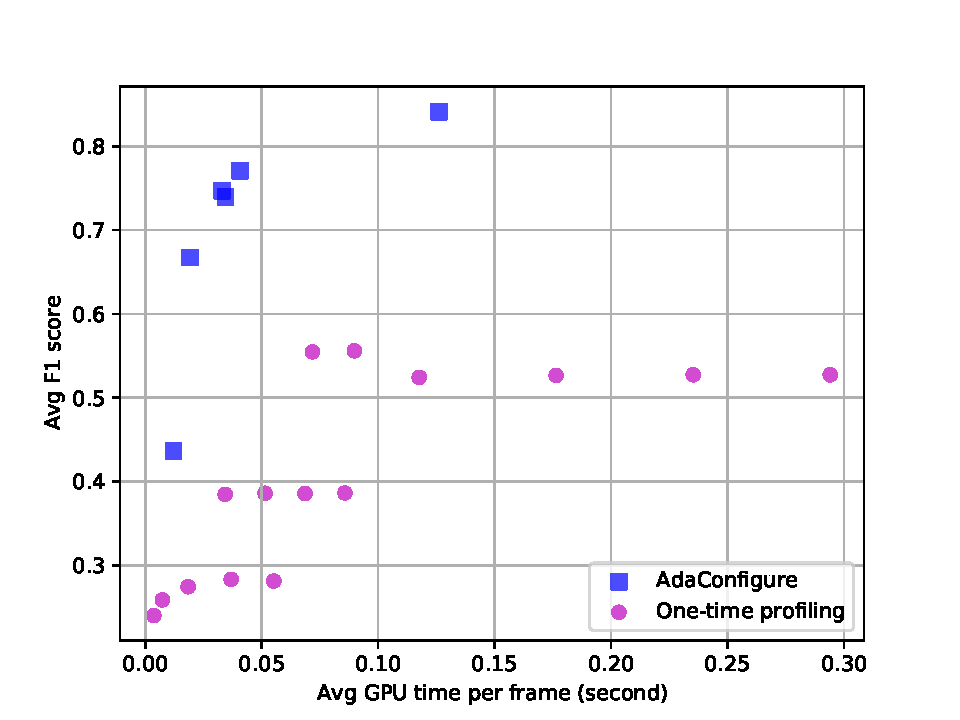
\includegraphics[width=5cm]{figures/Westbound.pdf}}
%		\centerline{(a) Camera 1 }%(Bounding box-based)}
%		\centerline{(Bounding box-based)}
%	\end{minipage}
%	\hfill
%	\begin{minipage}[t]{0.47\linewidth}
%		\centerline{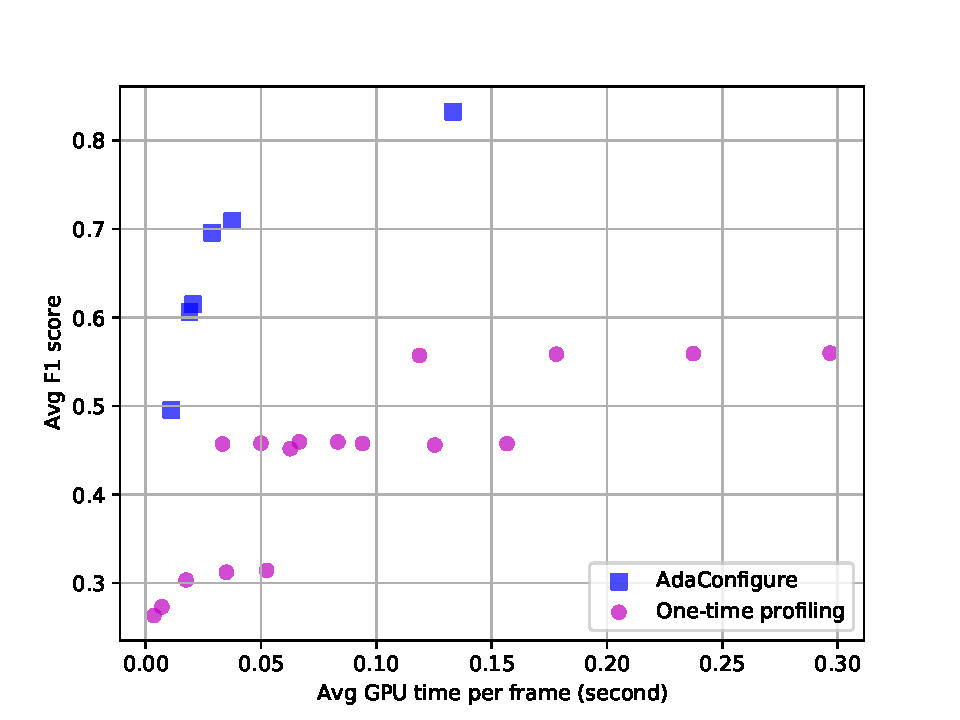
\includegraphics[width=5cm]{figures/Eastbound.pdf}}
%		\centerline{(b) Camera 2 }%(Bounding box-based)}
%		\centerline{(Bounding box-based)}
%	\end{minipage}
%	\vfill
%	\begin{minipage}[t]{\linewidth}
%		\centerline{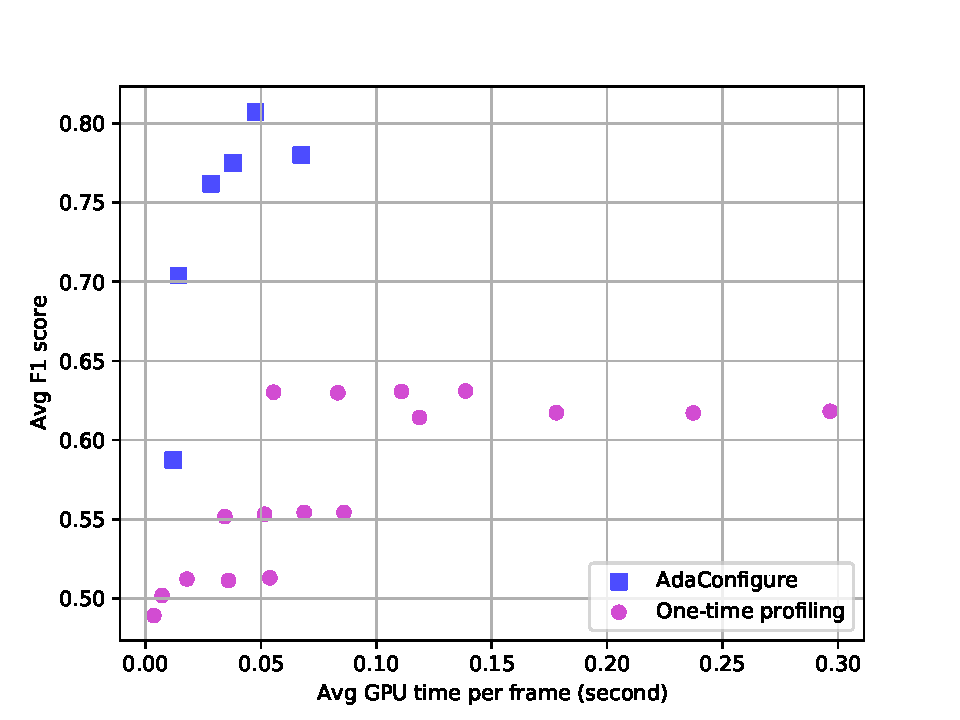
\includegraphics[width=5cm]{figures/Rear.pdf}}
%		\centerline{(c) Camera 3 }%(Bounding box-based)}
%		\centerline{(Bounding box-based)}
%	\end{minipage}		
%	\caption{AdaConfigure (blue) consistently outperforms the baseline of one-time profiling (magenta) across different cameras.}
%	\label{fig: 3dataset results}
%	%	\vspace{-0.5cm}
%\end{figure}
%
%To compare AdaConfigure's performance on single-camera inference and multi-camera inference, we respectively train and test the agent on each single-camera dataset of Multi-Camera Dataset. Figure \ref{fig: 3dataset results}(a)(b)(c) shows that AdaConfigure achieves 10-20\% higher accuracy with a similar amount of computation resources. 
%%or achieves similar accuracy with only 50-60\% of the computation resource on the single-camera inference. 
%As shown in Figure \ref{fig: results}(e), the gap between AdaConfigure and static configuration is larger than Figure \ref{fig: 3dataset results}(a)(b)(c), indicating that AdaConfigure has a better improvement on the multi-camera situation. AdaConfigure achieves 25-35\% higher accuracy with a similar amount of resources.
%%or reach higher accuracy with only 75-85\% of the resources on multi-camera inference.
%AdaConfigure achieves superior performance on multi-camera inference than single-camera inference. Instead of the static solution using fixed configuration in different situations, AdaConfigure can choose a proper configuration for different situations since the exact spatial characteristics of the video contents are different in different locations.


%It proves that our solution can pick the proper configuration according to intrusive dynamics of video contexts, including spatial and temporal features.

%\begin{figure*}[!t]
%	\begin{minipage}[t]{0.32\linewidth}
%		\centerline{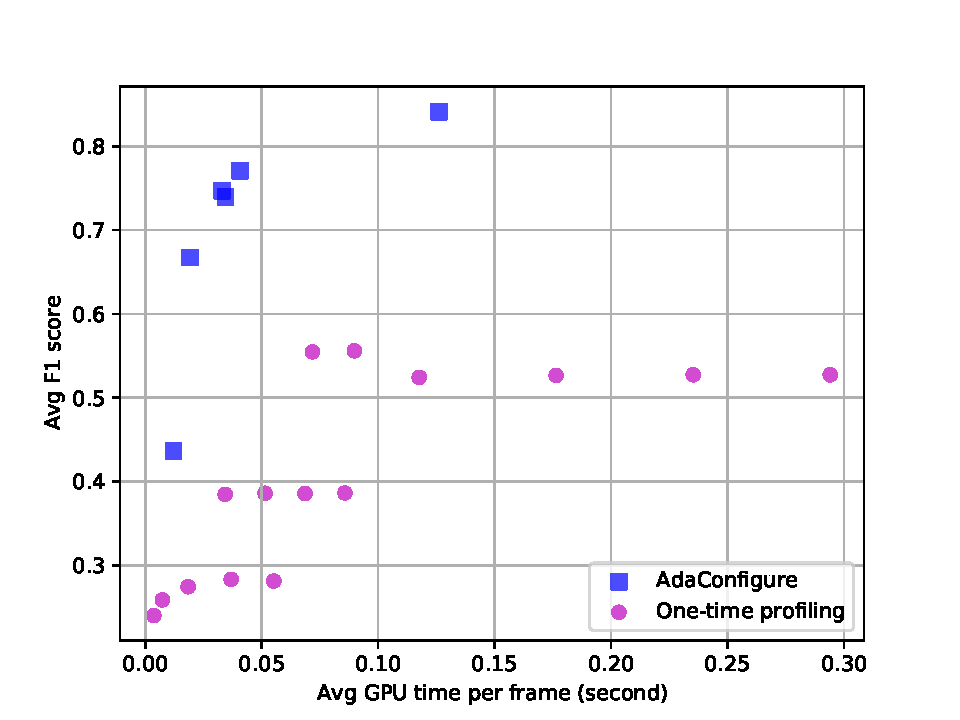
\includegraphics[width=6.5cm]{figures/Westbound.pdf}}
%		\centerline{(a) Camera 1 (Bounding box-based)}
%	\end{minipage}
%	\hfill
%	\begin{minipage}[t]{0.32\linewidth}
%		\centerline{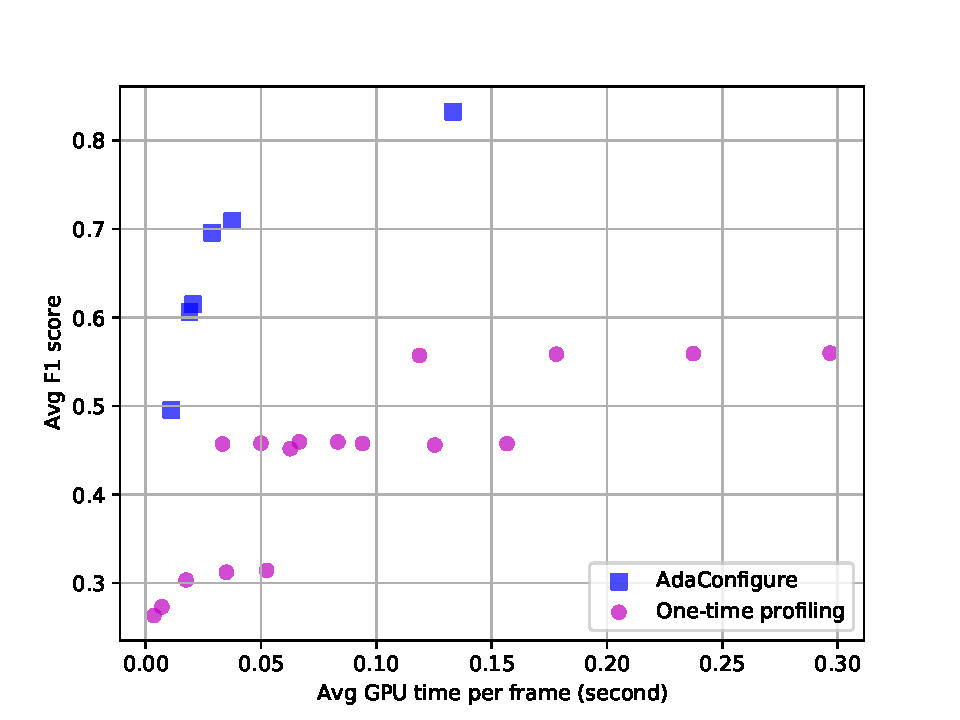
\includegraphics[width=6.5cm]{figures/Eastbound.pdf}}
%		\centerline{(b) Camera 2 (Bounding box-based)}
%	\end{minipage}
%	\hfill
%	\begin{minipage}[t]{0.32\linewidth}
%		\centerline{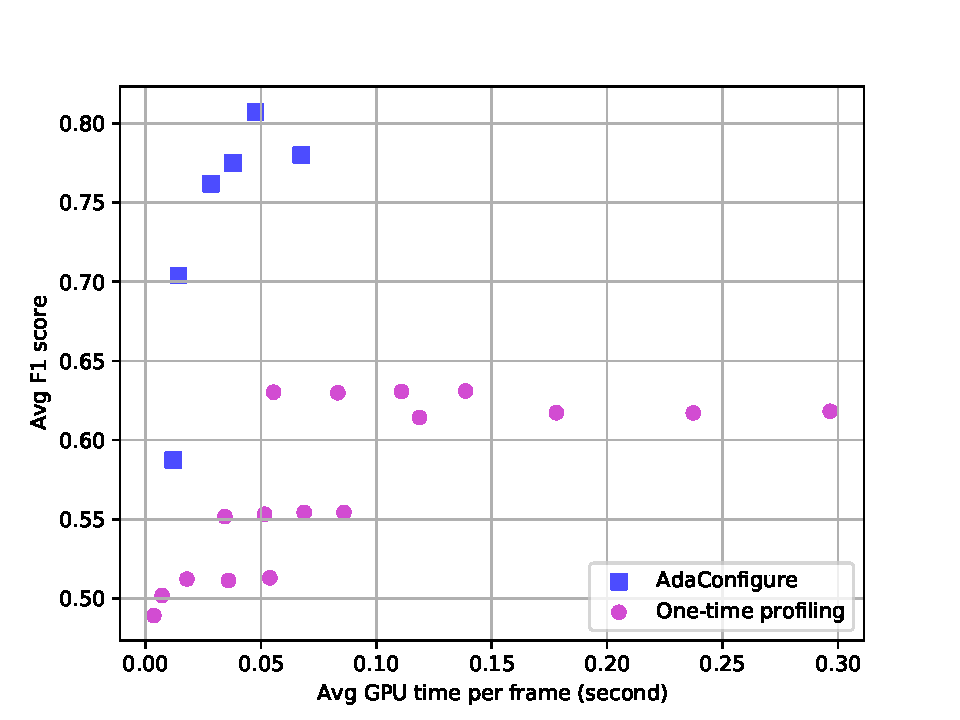
\includegraphics[width=6.5cm]{figures/Rear.pdf}}
%		\centerline{(c) Camera 3 (Bounding box-based)}
%	\end{minipage}		
%	\caption{AdaConfigure (blue) consistently outperforms the baseline of one-time profiling (magenta) across different cameras.}
%	\label{fig: 3dataset results}
%\end{figure*}
 
%\noindnet
 
\subsubsection{Low Profiling Cost of Adaptive Configuration}
\label{subsec: profiling cost}
%Comparing to the static solution that profiles configurations once, in our solution, the video
%chunk is passed to the AdaConfigure firstly to estimate the configuration. Running this RL agent brings profiling cost (extra resource consumption) to the whole system. 
%In this section, we evaluate this profiling cost. 
%In the inference phase, we divide the video into $T$-second intervals as video chunks and use AdaConfigure to choose the proper configuration for the first t seconds of the video chunk. It then sticks with the chosen configuration for the rest of the video chunk, i.e., for $T-t$ seconds. We use T = 4 and t = 1 for our experiments.
In our solution, the video chunk is passed to the AdaConfigure firstly to estimate the configuration, bringing profiling cost (extra resource consumption) to the whole system. 
The profiling cost, including the resource of extract $k_1$ embeddings and the cost of agent choosing actions. We test the average time on 30 hours video of Multi-Camera Dataset, and conclude that the average time of extract one embedding is 0.02s, and the average time of agent choosing action is 0.0006s, which can be ignored. We compute the ratio by dividing profiling time into total inference time as metric of profiling cost.
%, which is equals the frame number multiply the average time per frame. 
The profiling cost is about 0.2-2\% of the overall video analytics resource consumption. The concrete ratio depends on the concrete AdaConfigure configuration solutions, such as the solutions listed in Table \ref{tab: different sulutions}. For instance, when using the $\beta$ 0.7 solution, the profiling time is only 0.2\% of overall resource consumption on this solution; when using the $\beta$ 0.2 solution, the profiling cost is 1.5\%.        

\subsubsection{Different AdaConfigure Solutions to Meet Different Services}
\label{subsec: different sulutions}
In the training phase, when using different balance factors $\beta$ in the reward function, we would obtain different agents (different adaptive configuration strategies). 
%Each exact $\beta$ solution represents a concrete adaptive configuration strategy, which can adaptively update configuration across time. 
In general, the $\beta$ is bigger, indicating the accuracy is more important relatively, and the agent would choose a more expensive configuration. In our experiment, we set $\beta$ is 0.2,0.3,...,0.7, and the results of different AdaConfigure solutions on Multi-Camera Dataset are listed in Table \ref{tab: different sulutions}. 

\begin{table}[!t]
	\centering
	%     \begin{tabular}{lll}
	\resizebox{0.4\textwidth}{!}{
		\begin{tabular}{ccc}
			\toprule
			balance factor $\beta$ & Avg GPU time per frame (second) & Avg F1 score  \\ \midrule
			0.2          & 0.01384  &  0.64307            \\
			0.3          & 0.03314  &  0.72008            \\
			0.4          & 0.05203  &  0.79096            \\
			0.5          & 0.08479  &  0.80056            \\
			0.6          & 0.17570  &  0.87731            \\
			0.7          & 0.26511  &  0.93262            \\
			\bottomrule
	\end{tabular}}
	\caption{Resource consumption and bounding box-based F1 for different AdaConfigure solutions}
	\label{tab: different sulutions}
	%	\vspace{-0.1cm}
\end{table}

Table \ref{tab: different sulutions} shows that when the $\beta$ increases, the resource consumption and the accuracy of the corresponding solution would increase, indicating the AdaConfigure solutions of big $\beta$ would choose the more expensive configuration to inference. We can leverage this to train proper configuration strategy for different service demands, for example, using big $\beta$ for high-accuracy demand services and using small $\beta$ for low-accuracy demand services. 
%\begin{table}[!t]
%%\begin{table}[H]
%	\centering
%	%     \begin{tabular}{lll}
%	\resizebox{0.5\textwidth}{!}{
%		\begin{tabular}{lcc}
%			\toprule
%			Model and Image size & Inference time & Accuracy  \\ \midrule
%			SSD MobileNetV2 320p          & 49.5 ms  &  xxx            \\
%			SSD MobileNetV2 640p          & 58.5 ms  &  0.494            \\
%			SSD ResNet152V1 640p          & 100 ms  &  0.579            \\
%			SSD ResNet152V1 1024p          & 182.3 ms  &  0.614            \\
%			FasterRCNN ResNet50V1 640p          & 106.4 ms  &  0.637            \\
%			FasterRCNN ResNet50V1 1024p          & 120.5 ms  &  0.786           \\
%			FasterRCNN InceptionResNetV2 640p          & 361.8 ms  &  0.734            \\
%			FasterRCNN InceptionResNetV2 1024p          & 418.4 ms  &  1            \\
%			\bottomrule
%	\end{tabular}}
%	\caption{Inference time and F1 for different models and resolutions car truck}
%	\label{tab: latency-overhead}
%	% \vspace{-0.5cm}
%\end{table}
%
%\begin{table}[!t]
%	%\begin{table}[H]
%	\centering
%	%     \begin{tabular}{lll}
%	\resizebox{0.5\textwidth}{!}{
%		\begin{tabular}{lcc}
%			\toprule
%			Model and Image size & Inference time & Accuracy  \\ \midrule
%			SSD MobileNetV2 320p          & 49.5 ms  &  xxx            \\
%			SSD MobileNetV2 640p          & 58.5 ms  &  0.753            \\
%			SSD ResNet152V1 640p          & 100 ms  &  0.886            \\
%			SSD ResNet152V1 1024p          & 182.3 ms  &  0.942            \\
%			FasterRCNN ResNet50V1 640p          & 106.4 ms  &  0.889            \\
%			FasterRCNN ResNet50V1 1024p          & 120.5 ms  &  0.98           \\
%			FasterRCNN InceptionResNetV2 640p          & 361.8 ms  &  0.965            \\
%			FasterRCNN InceptionResNetV2 1024p          & 418.4 ms  &  1            \\
%			\bottomrule
%	\end{tabular}}
%	\caption{Inference time and F1 for different models and resolutions}
%	\label{tab: latency-overhead}
%	% \vspace{-0.5cm}
%\end{table}

%\begin{figure}[!t]
%	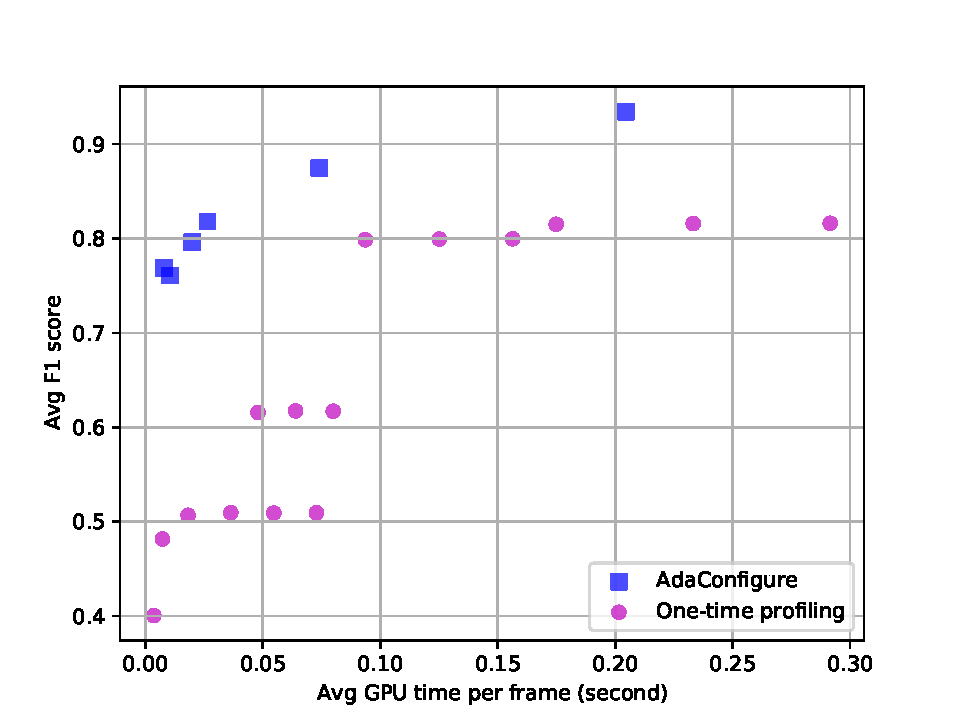
\includegraphics[width=9cm,height=8cm]{figures/m6.pdf}
%	\centering
%	\caption{The effect of different models, frame rate, and resolutions on accuracy and processing time. AdaConfigure (blue) consistently outperforms the baseline of one-time update (magenta) across different datasets. Each dot represents the results of running each solution.}
%	\label{fig_m6}
%\end{figure}
\section{Conclusion}
\label{Section: conclusion}

This paper proposes a reinforcement learning (RL)-based automatic video analytics configuration framework, AutoConfigure. Our solution can adapt the best configuration to intrusive dynamics of video contexts, meaning that it can periodically choose the proper configuration for the current video chunk according to the spatial and temporal correlation of video contexts. In the evaluation, AutoConfigure achieves 10-35\% higher accuracy with a similar amount of resources or achieves similar accuracy with only 50-85\% of the resources. AutoConfigure proves to be more efficient than static solutions and only creates an overhead of 0.1-1\% to the overall video analytics services.

% \section{Acknowledgments}

\bibliographystyle{IEEEbib}
\bibliography{ref}

\end{document}
